\documentclass[12pt]{article}
\usepackage[utf8]{inputenc}
\usepackage[numbers,sort&compress]{natbib}
\usepackage{amsmath,amssymb,amsfonts}
\usepackage{graphicx}
\usepackage{textcomp}
\usepackage{xcolor}
\usepackage{hyperref}
\usepackage{algorithm}
\usepackage{algpseudocode}
\usepackage{booktabs}
\usepackage{caption}
\usepackage{float}
\usepackage{geometry}
\usepackage{authblk}
\geometry{a4paper, margin=1in}

\hypersetup{
    colorlinks=true,
    linkcolor=blue,
    filecolor=magenta,      
    urlcolor=cyan,
}

% ========== TITLE & AUTHORS ==========
\title{\textbf{Dynamic Hybrid Forecasting Models for Drug Consumption Prediction in Hospital Pharmacies}}
\author[1,*]{Anping Guo}
\author[4,*]{Siye Wu}
\author[5,*]{Chiyu Wei}
\author[2,†]{Yuxin Fan}
\author[3,†]{Haizhu Tan}
\author[1]{Zhenzhen Pan}

\affil[1]{\small Department of Pharmacy, The First Affiliated Hospital of USTC, Division of Life Sciences and Medicine, University of Science and Technology of China, Hefei, China}
\affil[2]{\small University of Pennsylvania, Toronto, Ontario, Canada, M2N 6X5}
\affil[3]{\small Shantou University Medical College, Shantou, China, 515041}
\affil[4]{\small Independent Researcher, Toronto, Ontario, Canada, M2N 6X5}
\affil[5]{\small Zhongshan School of Medicine, Sun Yat-sen University, Guangzhou, China}


\date{}

\begin{document}

\maketitle

% ========== CORRESPONDING AUTHORS ==========
\noindent\textbf{† Corresponding Authors:} \\
Yuxin Fan, \texttt{yuxinfan@alumni.upenn.edu} \\
Haizhu Tan, \texttt{linnanqia@126.com} \\

\vspace{1ex}
\noindent\textbf{* These authors contributed equally}\\

\vspace{1ex}
\noindent\textbf{Email:} \\
Anping Guo, \texttt{guoanping@ustc.edu.cn} \\
Siye Wu, \texttt{april.siyewu@hotmail.com} \\
Yuxin Fan, \texttt{yuxinfan@alumni.upenn.edu} \\
Haizhu Tan, \texttt{linnanqia@126.com} \\
Chiyu Wei, \texttt{1535805000@qq.com} \\
Zhenzhen Pan, \texttt{panzhenzhencqmu@163.com} \\ 

\vspace{2ex}

% ========== ABSTRACT ==========
\maketitle

\newpage 
\begin{abstract}
Accurate and timely forecasting of drug consumption is critical for hospital pharmacies to maintain optimal inventory levels, minimize waste, and ensure continuous patient care. To address the challenges of temporal heterogeneity, seasonality, and irregular consumption patterns, we propose a performance-driven hybrid forecasting framework that dynamically selects the most suitable model—XGBoost, Prophet, or SARIMAX models based on rolling-window validation metrics. The framework exploits model-specific strengths, applying advanced feature engineering to tree-based learners and capturing autoregressive and seasonal dependencies in statistical time series models. By combining model selection with recent drug consumption dynamics, the proposed approach enhances predictive stability and accuracy across diverse drug consumption profiles. Empirical results demonstrate consistent improvements in forecasting performance, particularly under data sparsity and demand volatility.
\end{abstract}

\vspace{2ex}
\noindent\textbf{Keywords:} Drug Consumption Forecasting; Hospital Pharmacies; Forecasting Models; XGBoost; Prophet; SARIMAX

\vspace{3ex}

\section{Introduction}

Accurate forecasting of drug consumption is essential for effective management in hospital pharmacies~\cite{who2016}. By enabling optimal drug availability and mitigating the risks of overstocking or stockouts~\cite{fda2021}, reliable forecasts contribute significantly to reducing healthcare costs. Increasing studies~\cite{bhat2024optimizing}~\cite{koala2021factors} have emphasized the importance of demand forecasting in enhancing inventory efficiency and improving access to medication, especially within public healthcare systems.

Prophet, introduced by Taylor and Letham~\cite{taylor2018forecasting}, is a scalable forecasting model well-suited for large-scale time series applications. It effectively captures long-term trends and seasonality through changepoint detection. However, its performance can be sensitive to localized patterns and typically requires substantial parameter tuning. Moreover, its ability to incorporate exogenous variables is relatively limited. 

Extreme Gradient Boosting (XGBoost), developed by Chen and Guestrin~\cite{chen2016xgboost}, has achieved notable success in domains such as sales prediction and consumer behavior modeling, owing to its high flexibility and strong predictive power. However, when applied to time-series data like drug consumption, XGBoost may struggle to capture temporal dependencies due to its non-sequential, tree-based nature.

To address these limitations, more advanced models have been explored. For example, Meng et al.~\cite{meng2021comparative} demonstrate that Long Short-Term Memory (LSTM) excels at capturing long-term dependencies and modeling non-linear patterns in drug sales data. However, their applicability can be constrained by high computational demands. While Prophet remains effective in handling seasonal and holiday-related variations, its reliance on predefined trend assumptions can reduce adaptability in dynamic environments affected by sudden policy changes or epidemic outbreaks.

Xu et al.~\cite{xu2019hybrid} propose a hybrid forecasting framework that integrates a linear autoregressive model (auto-regression (AR) or auto-regressive integrated moving average (ARIMA)) with a Deep Belief Network (DBN), aiming to jointly capture linear trends and complex non-linearities. Although this method yields high prediction accuracy, it demands substantial computational resources and limited consideration of the influence of irregular external factors. 

Siddiqui et al. ~\cite{siddiqui2021hybrid} present ARIMA-Holt’s Winter (ARHOW), a composite model combining ARIMA with the Holt-Winters method to improve forecast accuracy. However, its reliance on fixed model architectures may reduce adaptability in settings characterized by rapid changes in demand patterns or external conditions.

Rathipriya et al. ~\cite{rathipriya2022pharma} develop a hybrid framework combining shallow neural networks (e.g., Radial Basis Function Neural Network, Generalized Regression Neural Network) and deep learning models (e.g., LSTM, Stacked LSTM). Their findings suggest that shallow networks are better suited for small and noisy datasets, while deep learning models offer superior performance in capturing temporal and non-linear dynamics, albeit with higher data and computational requirements.

In this study, we analyze monthly drug consumption data collected from hospital pharmacies over a span of nearly seven years, covering a wide range of drugs and manufacturers. The dataset exhibits significant variability due to seasonal effects, erratic demand patterns, and external factors such as policy interventions. These complexities highlight the limitations of conventional single-model forecasting approaches and underscore the need for more flexible and adaptive methods~\cite{lee2019}. 

To address these inherent complexities of hospital pharmacy demand data,we propose DynamicXSP, a hybrid forecasting framework specifically tailored to these real-world challenges. Rather than relying on a single model, DynamicXSP leverages the complementary strengths of multiple approaches: Prophet provides robust modeling of long-term seasonality; SARIMAX adjusts for exogenous factors and short-term shocks; and XGBoost captures non-linear dependencies and irregular demand patterns. These components are integrated through a rolling-window forecasting strategy, advanced feature engineering, and grid search optimization, enabling the framework to adapt dynamically to changing data regimes. While DynamicXSP is motivated by the distinct characteristics of regional pharmaceutical consumption data, its modular and model-agnostic architecture supports generalizability to other healthcare inventory or demand forecasting tasks with similar structural variability.

The remainder of this paper is arranged as follows: Section II introduces the research methodology and focuses on the advantages of the DynamicXSP framework. Section III presents the experiments and results, including data preprocessing and analysis. Finally, Section IV summarizes the study and outlines future directions on research.

\section{Methodology}
\subsection{DynamicXSP Model Framework}

 DynamicXSP follows a structured process:

\begin{itemize}
    \item Model training applies multiple models like SARIMAX, XGBoost and Prophet with automating grid search and rolling-window forecasting to ensure adaptability to recent trends.
    \item Feature engineering includes rolling statistics, lag-based variables and external factor indicators to enhance predictive modeling.
    \item Model selects the best one from multiple models based on the performance metrics such as \( R^2 \) and symmetric Mean Absolute Percentage Error (SMAPE)~\cite{hyndman2006accuracy}.
\end{itemize}

\begin{figure}[H]
    \centering
    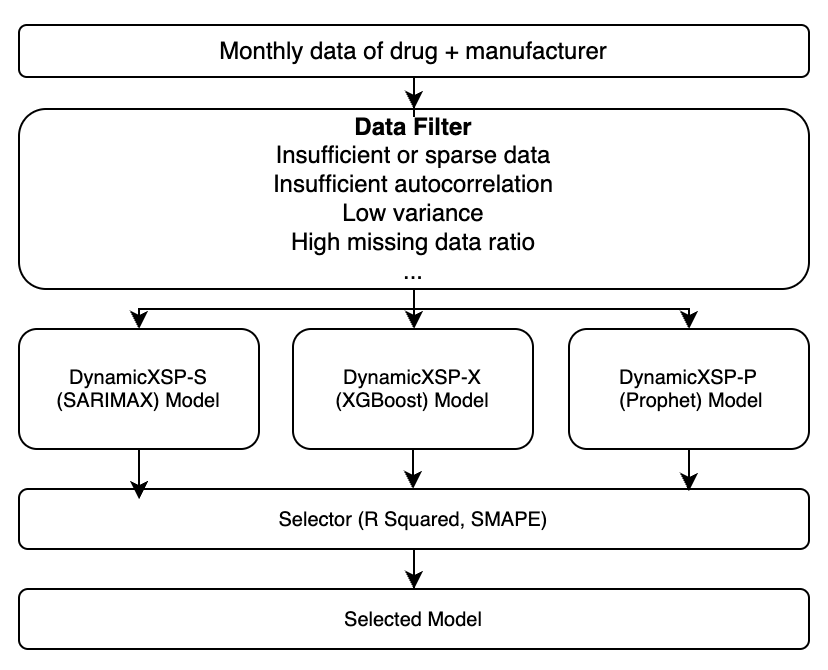
\includegraphics[width=\linewidth]{./model_structure.png}
    \caption{Model Structure of DynamicXSP Framework}
    \label{fig:vitaminb1}
\end{figure}

While unanticipated external shocks such as pandemics, climate or procurement policy~\cite{papadopoulos2024} shifts are difficult to capture without real-time external data, our framework emphasizes generalizability and low deployment cost. Selected variables are readily available in most hospital systems. The framework is extensible—XGBoost and Prophet both support custom regressors, and SARIMAX accommodates exogenous inputs—allowing easy integration of richer data sources when available, as explored in healthcare forecasting studies~\cite{li2023,zhang2021}.

\subsection{Model Design and Roles}
\subsubsection{DynamicXSP-S (SARIMAX) Model}

This approach considers not only historical trends but also external influences such as manufacturer supply patterns and drug inventory policies at hospital. The model is defined as below:

\begin{equation}
    \hat{y}_{t} = \phi(B)\theta(B)^{-1} \left( c + \mathbf{X}_{t}\beta + \epsilon_{t} \right),
\end{equation}

where \(y_{t}\) represents the weekly drug inventory consumption, \(\mathbf{X}_{t}\) represents the set of exogenous features designed to capture the relevant consumption patterns, and \(\epsilon_{t}\) is a white noise error term.

To improve prediction accuracy, the DynamicXSP-S model includes specific feature engineering tailored to hospital pharmacy demand. These features take both short-term fluctuations and long-term trends, improving the adaptability of the model in dynamic environments. The main engineered features include:

\begin{itemize}
    \item Lagged value: captures the delayed effect of past consumption, especially suitable for modeling hospital replenishment cycles and manufacturer supply constraints:
    \begin{equation}
    \text{drug\_consume\_lag}_{k} = y_{t-k}, \quad k \in \{1, 3, 6, 12\}.
    \end{equation}
    The lag selections is consistent with common drug purchase intervals in historical data.

    \item Rolling statistics: represent short-term demand fluctuations and variations and help the model explain unexpected spikes in drug use due to policy changes or seasonal illnesses:
    \begin{align}
    \text{consume\_rolling\_mean}_{k} &= \frac{1}{k} \sum_{i=1}^{k} y_{t-i}, \\
    \text{consume\_rolling\_std}_{k} &= \sqrt{\frac{1}{k} \sum_{i=1}^{k} (y_{t-i} - \text{mean})^2}.
    \end{align}
    Unlike standard moving averages, these rolling features are dynamically adjusted to ensure adaptability across different drug types and manufacturers.

    \item Seasonality encoding: Due to hospital procurement schedules, drug consumption often follows predictable monthly cycles. To simulate this effectively, we employ trigonometric transformations:
    \begin{align}
    \text{month\_sin} &= \sin\left(\frac{2\pi \cdot \text{month}}{12}\right), \\
    \text{month\_cos} &= \cos\left(\frac{2\pi \cdot \text{month}}{12}\right).
    \end{align}
    This formulation enables SARIMAX to smoothly capture periodic fluctuations without manually performing seasonal differencing~\cite{box2015}.

    \item Exponentially Weighted Moving Average (EWMA): Introduces a memory-adjusted smoothing technique that prioritizes recent observations, making the model more responsive to sudden shifts in drug demand:
    \begin{equation}
    \text{EWMA}_{\alpha} = \alpha y_{t} + (1-\alpha) \cdot \text{EWMA}_{\alpha,t-1}.
    \end{equation}
    The smoothing factor \(\alpha\) is adjusted according to the specific volatility of drug (in our model, we use 3), to ensure that short-term demand peaks are reflected in the model while filtering out noise.

    \item Percentage change and trend strength: Designed to measure relative variations and stability in consumption patterns, providing key signals for adaptive inventory planning:
    \begin{align}
    \text{pct\_change\_consume}_{k} &= \frac{y_{t} - y_{t-k}}{y_{t-k}}, \\
    \text{comsume\_trend\_strength} &= \frac{1}{k} \sum_{i=1}^{k} \lvert y_{t-i} - y_{t-i-1} \rvert.
    \end{align}
    The trend strength metric allows the model to differentiate between regular seasonal variations and abrupt changes due to supply chain disruptions.
\end{itemize}

These features were selected through statistical analysis of hospital pharmacy consumption data, ensuring that the SARIMAX model effectively captures both recurring demand patterns and unexpected fluctuations. By incorporating rolling-window forecasting and dynamically adjusting feature selection for each drug-manufacturer pair, our approach improves predictive accuracy and enhances robustness in real-world hospital inventory management.

\subsubsection{DynamicXSP-X (XGBoost) Model}

XGBoost is a gradient boosting framework that constructs an ensemble of decision trees to predict the target variable \(y_t\). It excels in time-series forecasting, particularly for data with non-linear relationships and sparsity, making it well-suited for predicting drug consumption, where demand varies across manufacturers and fluctuates due to external factors. The model predicts \(y_t\) through an additive function:

\begin{equation}
\hat{y}_{t} = F(x_{t}) = \sum_{k=1}^{K} f_{k}(x_{t}), \quad f_{k} \in \mathcal{F},
\end{equation}

where \(\hat{y}_{t}\) is the predicted value, \(x_{t}\) represents input characteristics, \(f_{k}\) represents the \(k\)-th decision tree, and \(\mathcal{F}\) is the space of decision trees.

To effectively model time dependencies, the DynamicXSP-X framework incorporates lagged values (\(y_{t-1}, y_{t-2}, \dots\)), rolling statistics (such as moving averages and standard deviations over 3, 6, and 12 periods), and indicators reflecting consumption trends. These engineering features enable the model to identify historical patterns of drug usage and detect changes in demand, which is crucial given the variation across manufacturers. Additionally, the interaction terms between lagged values and rolling statistics further enhance the ability of the model to capture advanced dependencies.

The key hyperparameters, including the number of estimators, tree depth, learning rate and sampling ratios, are optimized by grid search to strike a balance between accuracy and computational efficiency. As part of the hybrid forecasting framework, DynamicXSP-X continuously updates its training data, ensuring adaptability to changing demand patterns.

DynamicXSP-X complements statistical models like DynamicXSP-S by capturing non-linear interactions and irregular consumption trends. It is able to learn intricate patterns from historical data, making it a adaptive and robust component in the prediction system.

\subsubsection{DynamicXSP-P (Prophet) Model}

Prophet is a time-series forecasting model, designed to decompose data into trend, seasonality, and external event components~\cite{kwarteng2024prophet}. In our model, we optimized Prophet to DynamicXSP-P to make it more effective for handling missing values, outliers, and irregular consumption patterns for drug demand forecasting, where sudden fluctuations and manufacturer-specific trends are common. The model predicts the target variable \(y_t\) as:

\begin{equation}
y_{t} = g(t) + s(t) + h(t) + \epsilon_{t},
\end{equation}

where \(g(t)\) represents a long-term trend, \(s(t)\) captures seasonal patterns using Fourier series, \(h(t)\) considers external disturbances (such as supply chain delays or regulatory policy changes), and \(\epsilon_{t}\) is the white noise error term. This decomposition enhances interpretability while allowing the model to dynamically adjust to various consumption behaviors.

The key hyperparameters are optimized to ensure that the model can effectively adapt to changes in drug demand. The adjustment process focuses on:
\begin{itemize}
    \item \textit{seasonality\_mode}: Determines whether seasonal effects are additive or multiplicative, based on consumption volatility.
    \item \textit{changepoint\_prior\_scale}: Controls the sensitivity to sudden trend changes, which are essential to model demand surgency or supply disruptions.
    \item \textit{seasonality\_prior\_scale}: Adjusts the weights of seasonal components to ensure a balance between smooth short-term variations and long-term trends.
\end{itemize}
The higher \textit{changepoint\_prior\_scale} value allows the model to react more quickly to structural changes, such as increased demand due to new hospital procurement policies, while lower values favor smoother trend transitions.

DynamicXSP-P benefits from continuous data updates, allowing it to react responsive to changing drug consumption trends while preventing overfitting outdated patterns. Through leveraging decomposition-based prediction and hyperparameter tuning, Prophet provides an interpretable prediction mechanism that is complementary to DynamicXSP-S and DynamicXSP-X within the hybrid framework. Its ability to capture trend changes and seasonal dependencies makes it an important component to improve the forecasting accuracy of various drug manufacturers.


\subsection{Dynamic Rolling-Window Forecasting}
To adapt to dynamic consumption patterns, a rolling-window mechanism is implemented~\cite{liu2020}. At each prediction step $t$, the model is trained using historical data $\{y_1, y_2, \ldots, y_t\}$, and the prediction for $t+1$ is made. The window then updates to include the latest observation, ensuring that the model adapts to recent trends.

Time-series data in drug consumption prediction usually exhibit non-stationarity, that is, trends, seasonality, and noise update over time. Static prediction methods that rely on fixed historical data may struggle to capture these dynamics, resulting in poort performance. To address this issue, a dynamic rolling-window forecasting strategy is applied, which enables models to prioritize recent information and adapt to structural changes in demand.

At each time step \(t\), the training dataset is updated to include the most recent observations, while discards older data beyond the defined window size (\(W\)). In detail, the training dataset at \(t\) is defined as follows:

\[
\mathcal{D}_{t} = \{(y_{\tau}, \mathbf{X}_{\tau}) \mid \tau \in [t - W, t-1]\},
\]

where \(\mathcal{D}_{t}\) is the training data, \(y_{\tau}\) represents the target variable (drug consumption), and \(\mathbf{X}_{\tau}\)  denotes the corresponding feature vectors. After training on \(\mathcal{D}_{t}\), a prediction is made for the next time step (\(t+1\)).

The rolling-window approach effectively captures short-term dynamics by prioritizing recent patterns while reducing the impact of outdated data. This is particularly beneficial for dealing with structural changes such as sudden demand breaks due to hospital procurement cycles, supply fluctuations by different manufacturers, and regulatory interventions. The choice of window size (\(W\)) is critical: larger windows contain long-term trends, while smaller ones emphasize recent changes. This study evaluates a variety of window sizes and selects the best configuration based on metrics such as root mean squared error (RMSE) and symmetric mean absolute percentage error (SMAPE)~\cite{hyndman2018}.

The rolling-window forecasting in the hybrid framework enhances adaptability:
\begin{itemize}
    \item \textbf{DynamicXSP-S}: Dynamically recalibrates coefficients to model short-term dependencies and external effects in drug consumption.
    \item \textbf{DynamicXSP-X}: Refines the decision tree with updated feature interactions that capture evolving non-linear relationships in manufacturer-specific demand shifts.
    \item \textbf{DynamicXSP-P}: Updates the trend decomposition to be consistent with the latest data, to ensure better adaptation to structural and seasonal changes.
\end{itemize}

While a fixed window size may not perfectly adapt to all drug types, we address this limitation by empirically selecting the window size based on category and volatility during the training phase. Additionally, we apply smoothing strategies such as moving averages to balance short- and long-term trends. Adaptive windowing was avoided to prevent overfitting and model instability.

This iterative strategy ensures that the model remains responsive and resilient to change, achieving predictive performance across different drug consumption scenarios by continuously adapting to the latest data trends.


\section{Experiments}

\subsection{Dataset}
The dataset in this study consists of monthly drug consumption records collected from two hospital pharmacies between January 1, 2018, and September 1, 2024, in China. These two hospitals are the First Affiliated Hospital of USTC and Anhui Cardiovascular and Cerebrovascular Hospital. The data includes a wide range of drugs across multiple categories and manufacturers, consisting of 542 combinations of drugs and manufacturers. Each record contains the manufacturer, drug name, monthly consumption value, inventory level, and proportions and trends. 

\subsection{Data Pre-processing Pipeline}
To ensure data consistency and quality, missing values in key features were interpolated where possible. Besides, records with excessive missing data were excluded with a sparsity threshold at 0.7 to maintain dataset integrity.

Outlier detection was conducted using a rolling window approach. For each drug-manufacturer combination, rolling statistics such as mean and standard deviation were calculated over a seven-month window. Values above three standard deviations from the mean or beyond the 5th and 95th percentiles were marked as outliers and adjusted to boundary values to maintain the time series' continuity.

To let the dataset contains only high-quality samples for modeling, we evaluated the temporal autocorrelation of consumption data and removed groups failing to exhibit sufficient autocorrelation. Other filtering criteria include variance thresholds and skewness limits to avoid heavily unbalanced target distributions.

Feature engineering was also performed to improve the predictive power. Some derived features such as lagged consumption values (e.g., previous month’s consumption), rolling statistics (e.g., mean, variance, and percent changes), and seasonal indicators encoded in trigonometric functions were created to capture time dependencies and periodic trends. These steps ensured that the final dataset was informative, robust and well-suited for downstream predictive modeling tasks.


\subsection{Data Analysis}

To improve the effectiveness of forecasting models on drug consumption, we implemented the DynamicXSP model framework. Each model in DynamicXSP was applied to forecast sales data across a diverse set of drugs and manufacturers. The dataset comprised monthly time series data spanning seven years, capturing trends, seasonality, and irregular fluctuations in drug consumption. 

The selection of the optimal model within DynamicXSP for each drug-manufacturer pair was conducted through an exhaustive grid search over the hyperparameter space, systematically evaluating various configurations to maximize predictive performance. The final model selection criterion was based on achieving the highest $R^2$ while minimizing SMAPE, ensuring both accuracy and robustness. By leveraging grid search, we identified the most effective parameter combinations for each drug and manufacter combination, optimizing both trend adaptation and error reduction across different demand patterns.


\subsection{Model Results}
\subsubsection{Representative Drug Cases}

\paragraph{DynamicXSP-X (XGBoost) Model} 
\begin{itemize}
\item \textbf{Drug:} Mycophenolate Sodium Enteric Tablets
\begin{itemize}
\item \textbf{Manufacturer:} Novartis Switzerland
\item \textbf{Metrics:} $R^2 = 0.8154$, SMAPE = 25.40
\end{itemize}

Figure \ref{fig:mycophenolate} illustrates the prediction performance of DynamicXSP-X (XGBoost) for Mycophenolate Sodium Enteric Tablets. The model effectively captured complex non-linear demand fluctuations, particularly during the volatile periods of 2023-2024. With a high $R^2$ of 0.8154, it demonstrated strong predictive accuracy in tracking consumption trends, while the SMAPE of 25.40 suggests a relatively low forecasting error despite market fluctuations.

\begin{figure}[H]
\centering
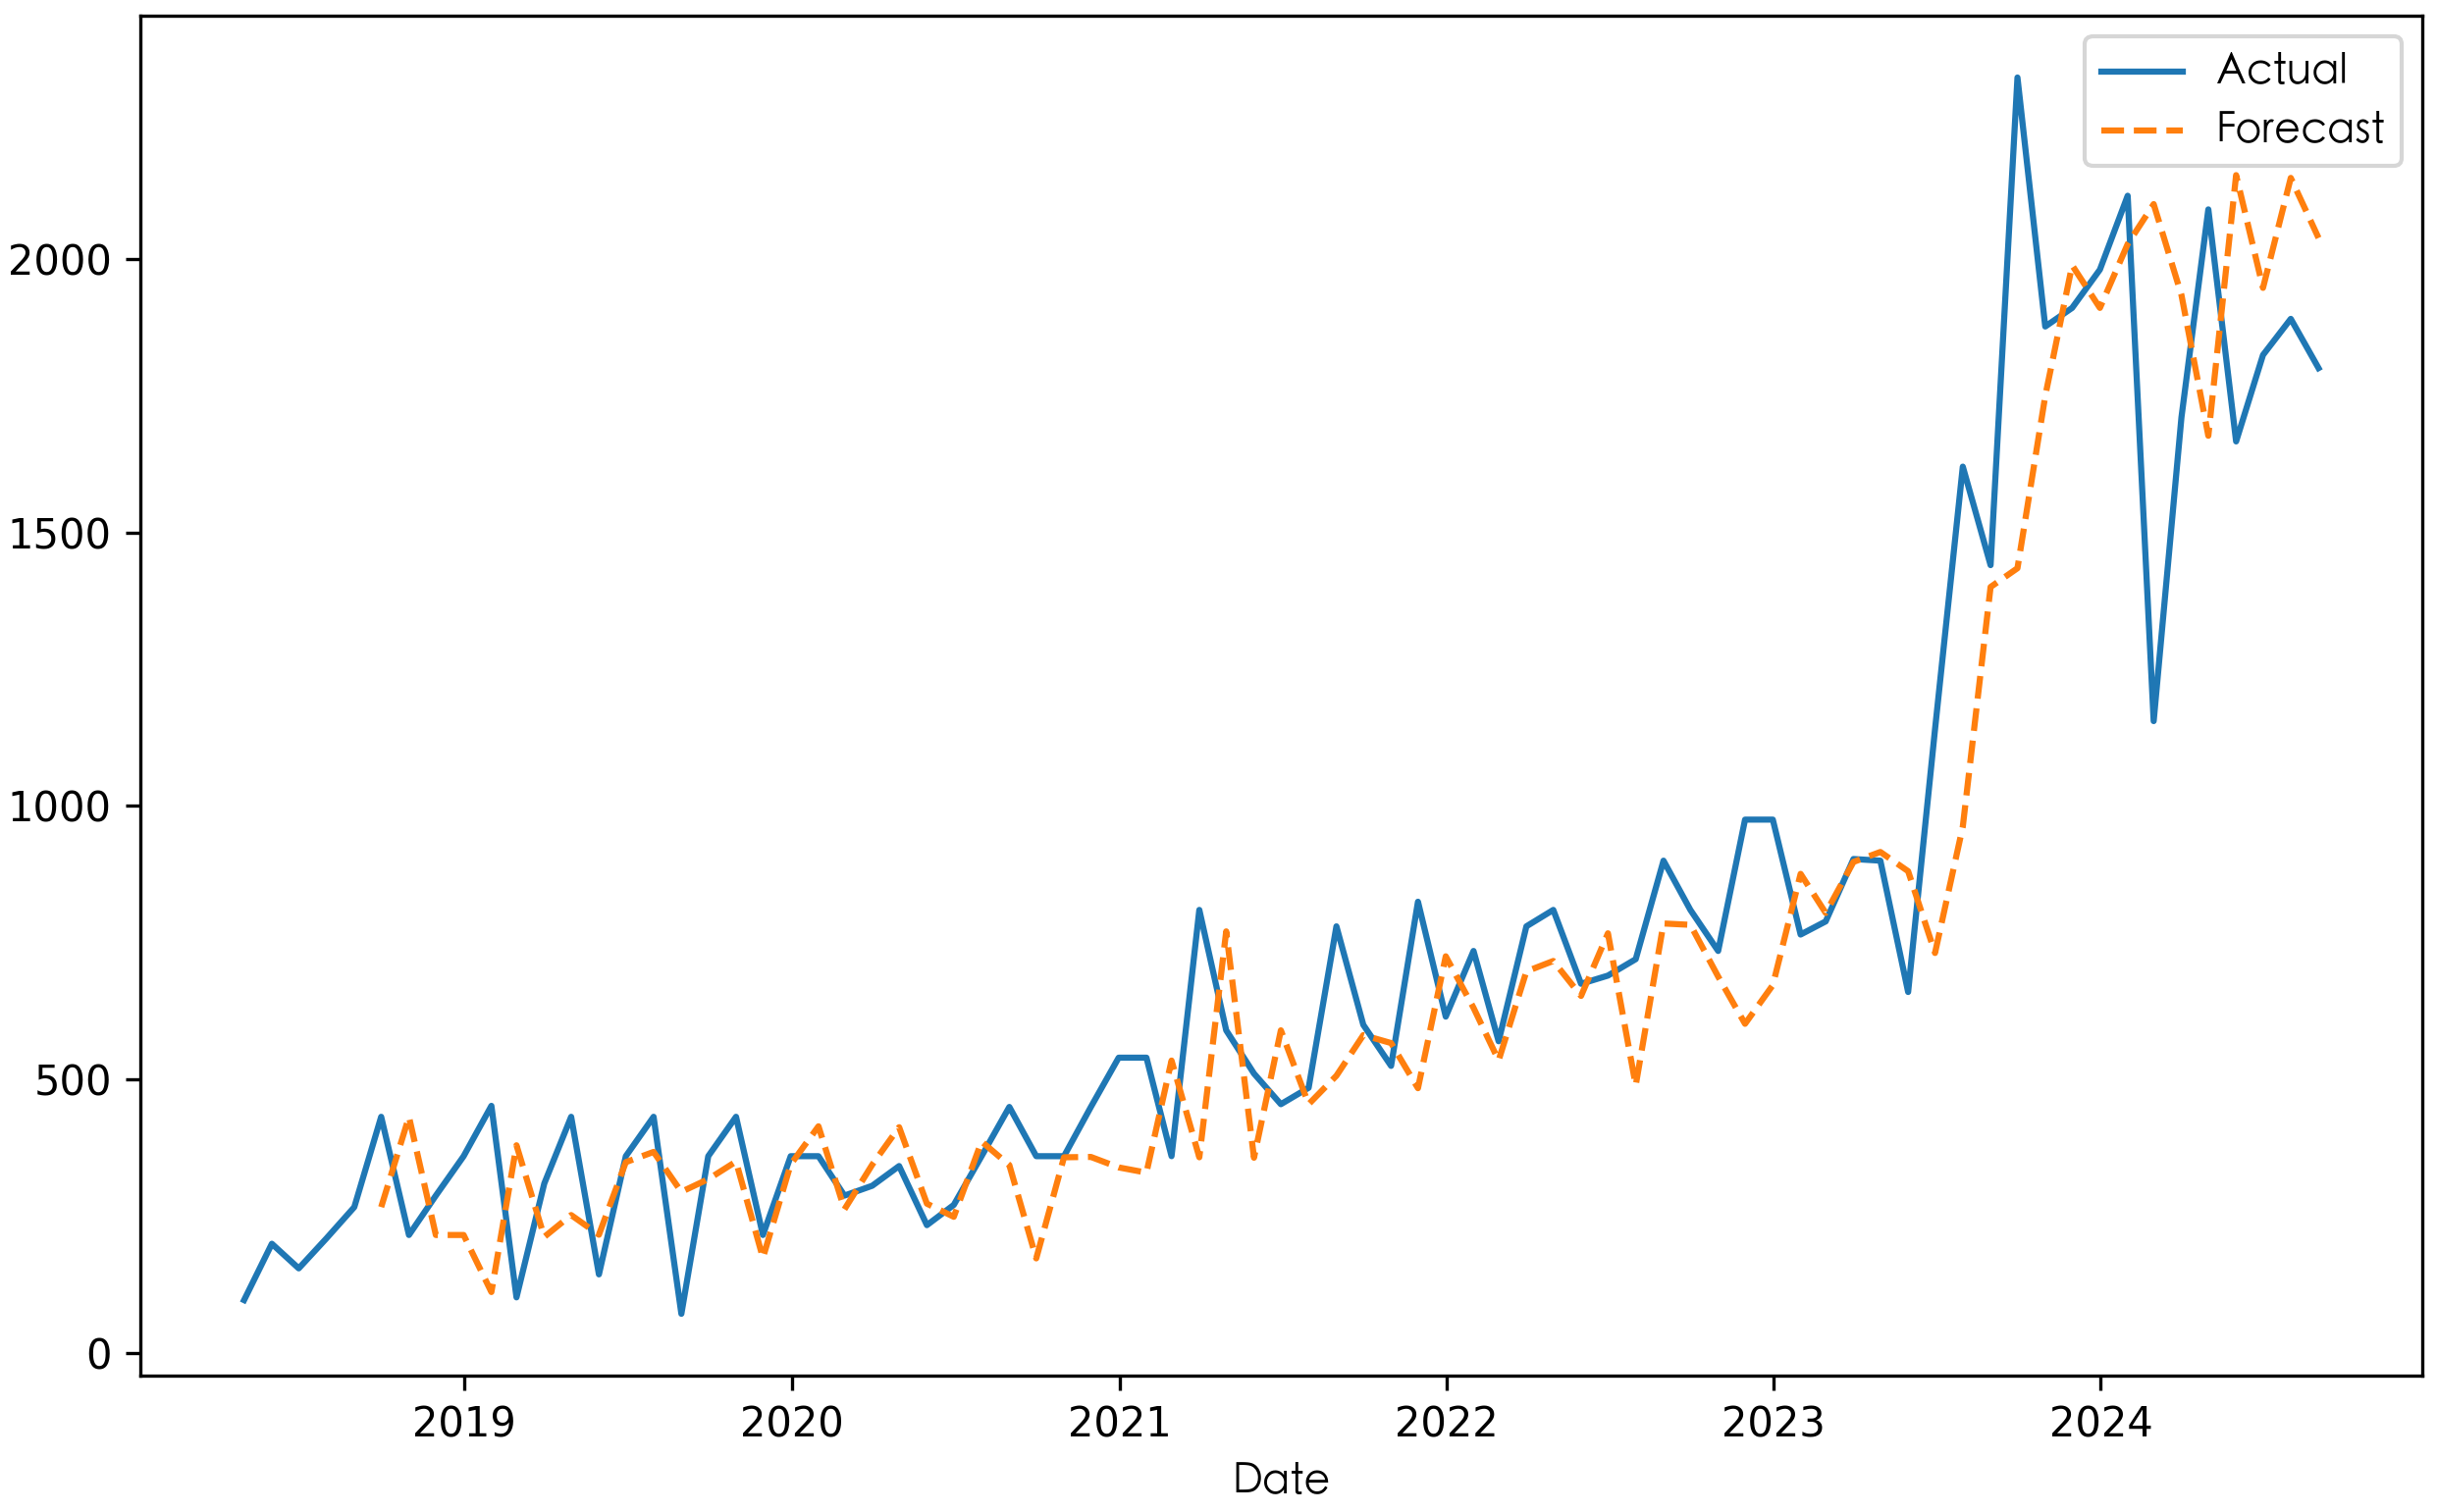
\includegraphics[width=\linewidth]{../Result_Paper/XGBoost_Prediction_麦考酚钠肠溶片_瑞士诺华.png}
\caption{DynamicXSP-X (XGBoost) Model Prediction for Mycophenolate Sodium Enteric Tablets by Novartis.}
\label{fig:mycophenolate}
\end{figure}
\item \textbf{Drug:} Flurbiprofen Gel Patch
\begin{itemize}
\item \textbf{Manufacturer:} Jingtaide
\item \textbf{Metrics:} $R^2 = 0.7902$, SMAPE = 21.14
\end{itemize}
Figure \ref{fig:flurbiprofen} presents the forecast results for Flurbiprofen Gel Patch. DynamicXSP-X effectively captured the increasing trend and high volatility in demand. The model achieved an $R^2$ of 0.7902, indicating strong trend alignment, while a SMAPE of 21.14 highlights its ability to maintain low relative errors even in fluctuating market conditions.
\begin{figure}[H]
\centering
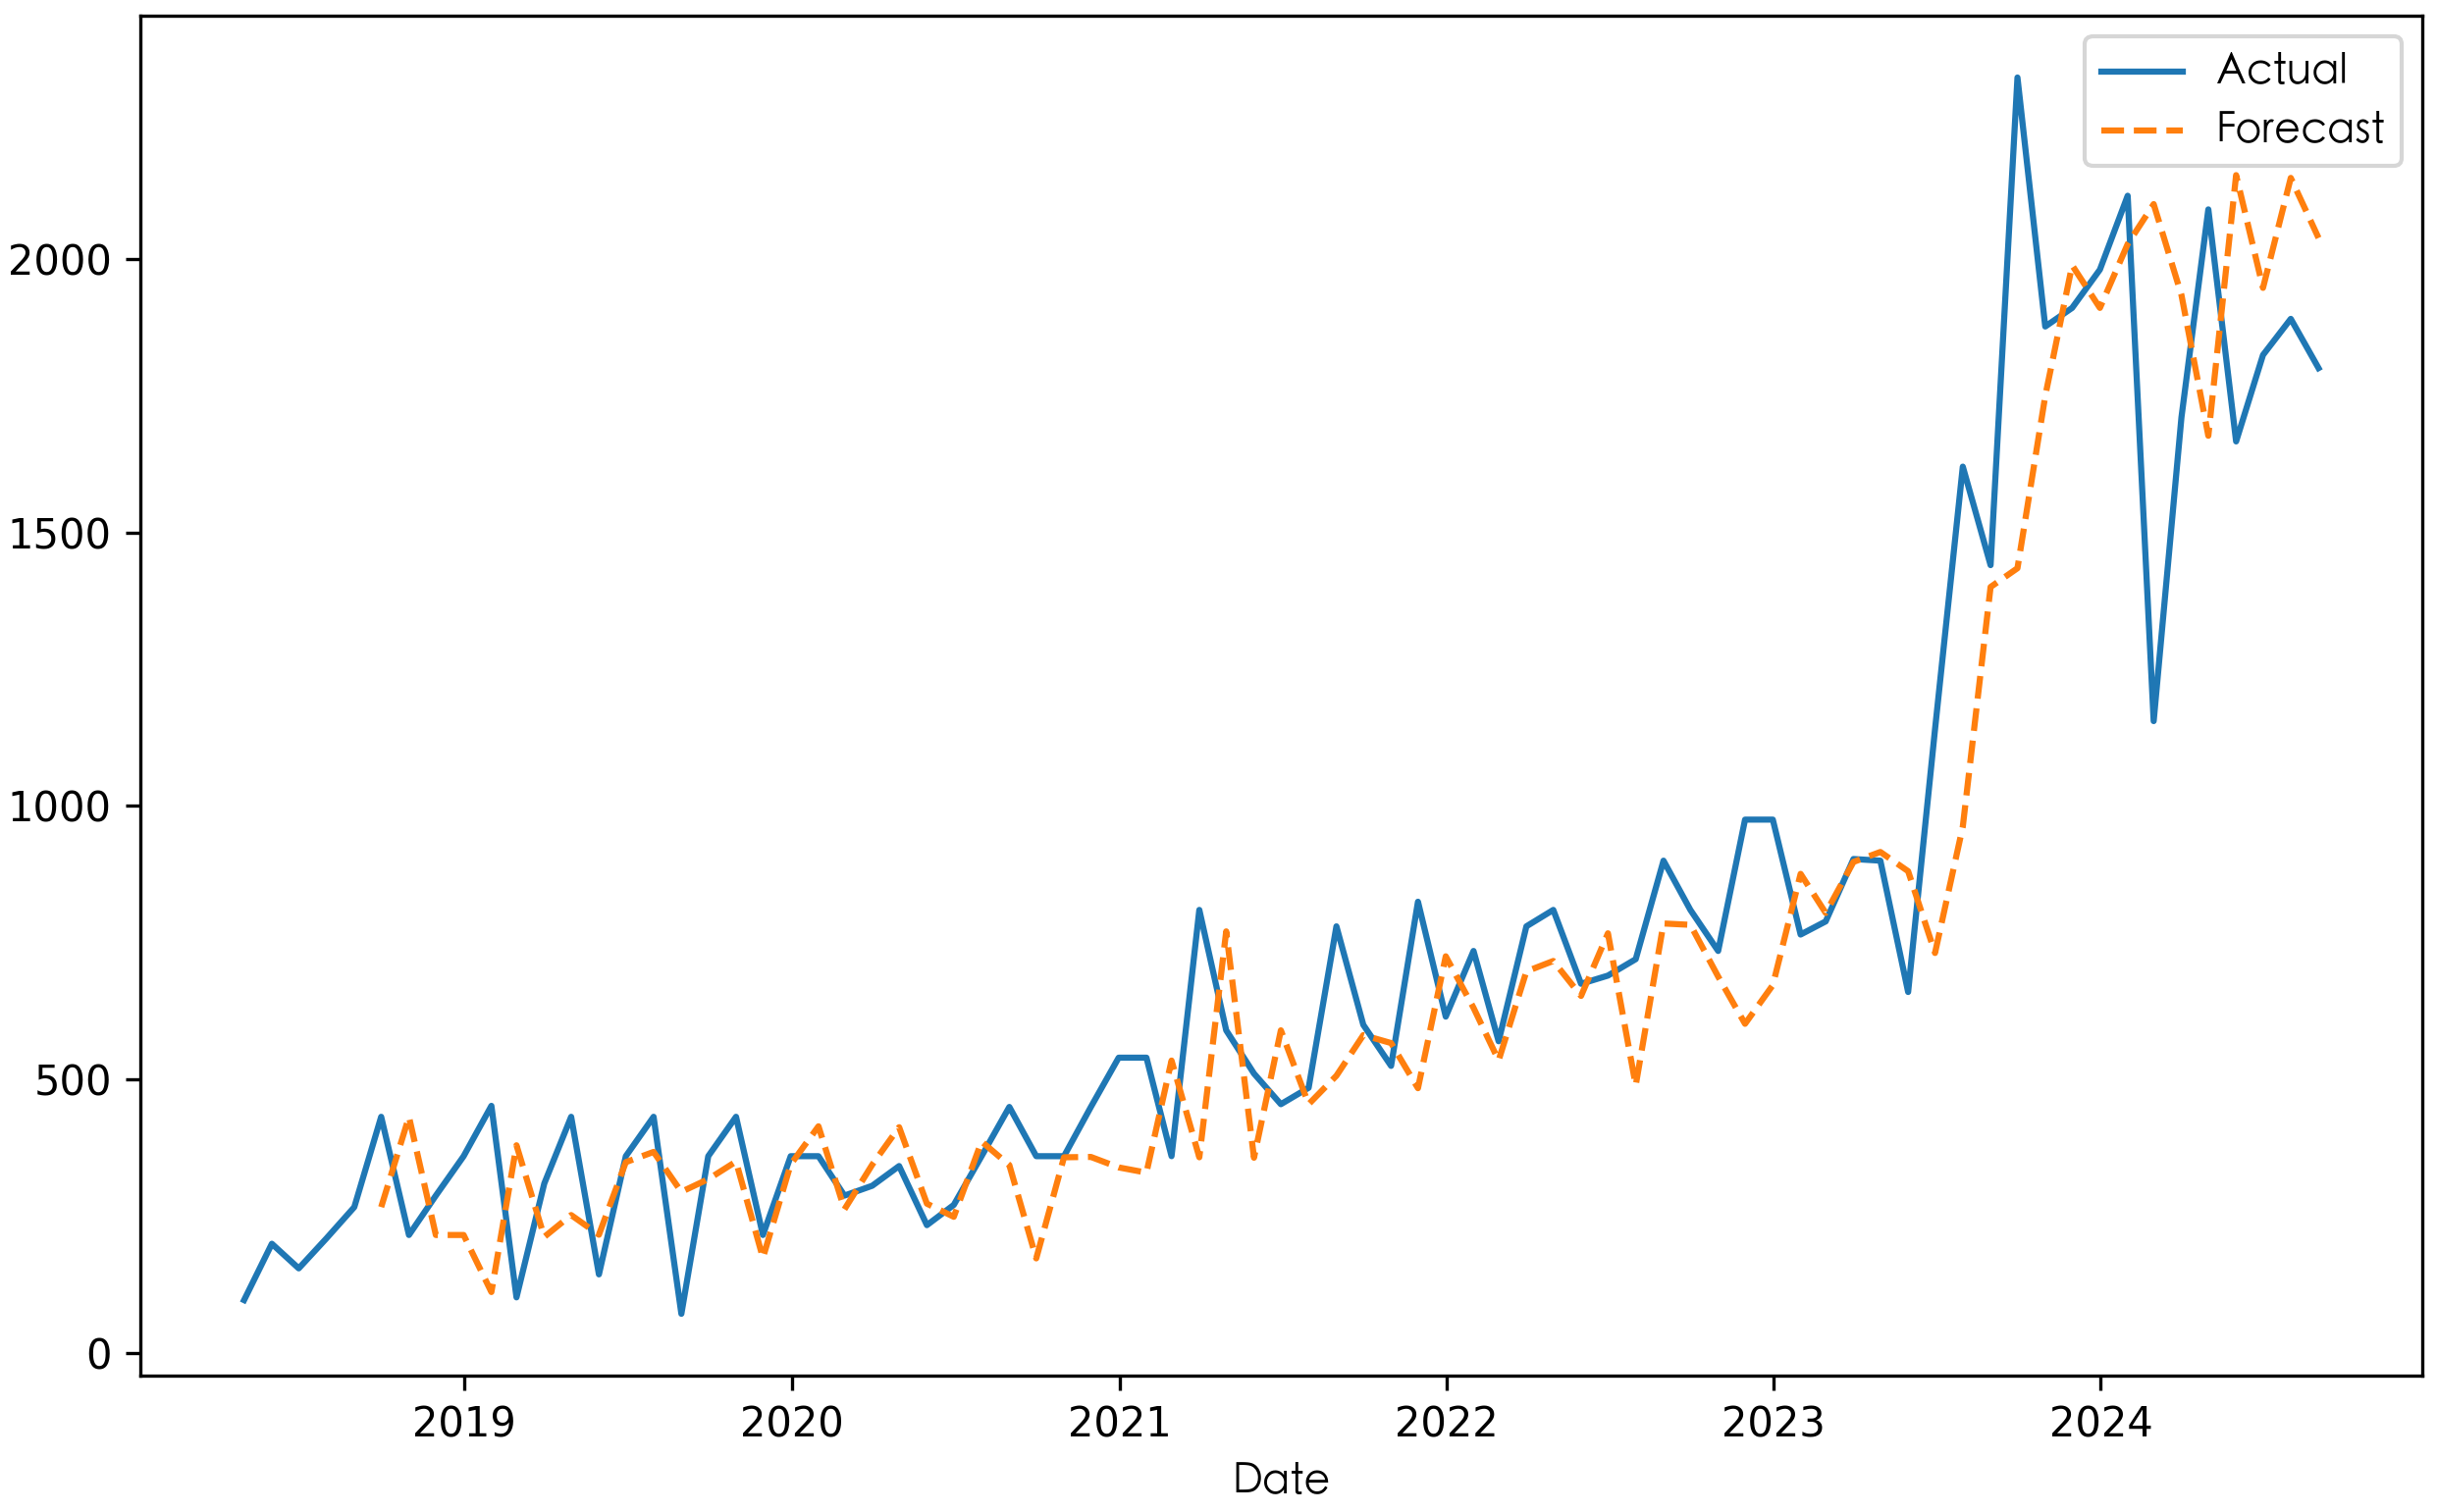
\includegraphics[width=\linewidth]{../Result_Paper/XGBoost_Prediction_麦考酚钠肠溶片_瑞士诺华.png}
\caption{DynamicXSP-X (XGBoost) Model Prediction for Flurbiprofen Gel Patch by Jingtaide.}
\label{fig:flurbiprofen}
\end{figure}
\end{itemize}

\paragraph{DynamicXSP-P (Prophet) Model}
\begin{itemize}
\item \textbf{Drug:} Compound Phellodendron Liquid
\begin{itemize}
\item \textbf{Manufacturer:} Lu Hanfang
\item \textbf{Metrics:} $R^2 = 0.7898$, SMAPE = 22.63
\end{itemize}
Figure \ref{fig:phellodendron} depicts the prediction results of DynamicXSP-P (Prophet) for Compound Phellodendron Liquid. The model effectively captured long-term trend patterns and seasonal fluctuations, as reflected in its strong $R^2$ value of 0.7898. The SMAPE of 22.63 indicates a balanced trade-off between accuracy and stability, demonstrating the model's ability to manage periodic demand spikes.
\begin{figure}[H]
\centering
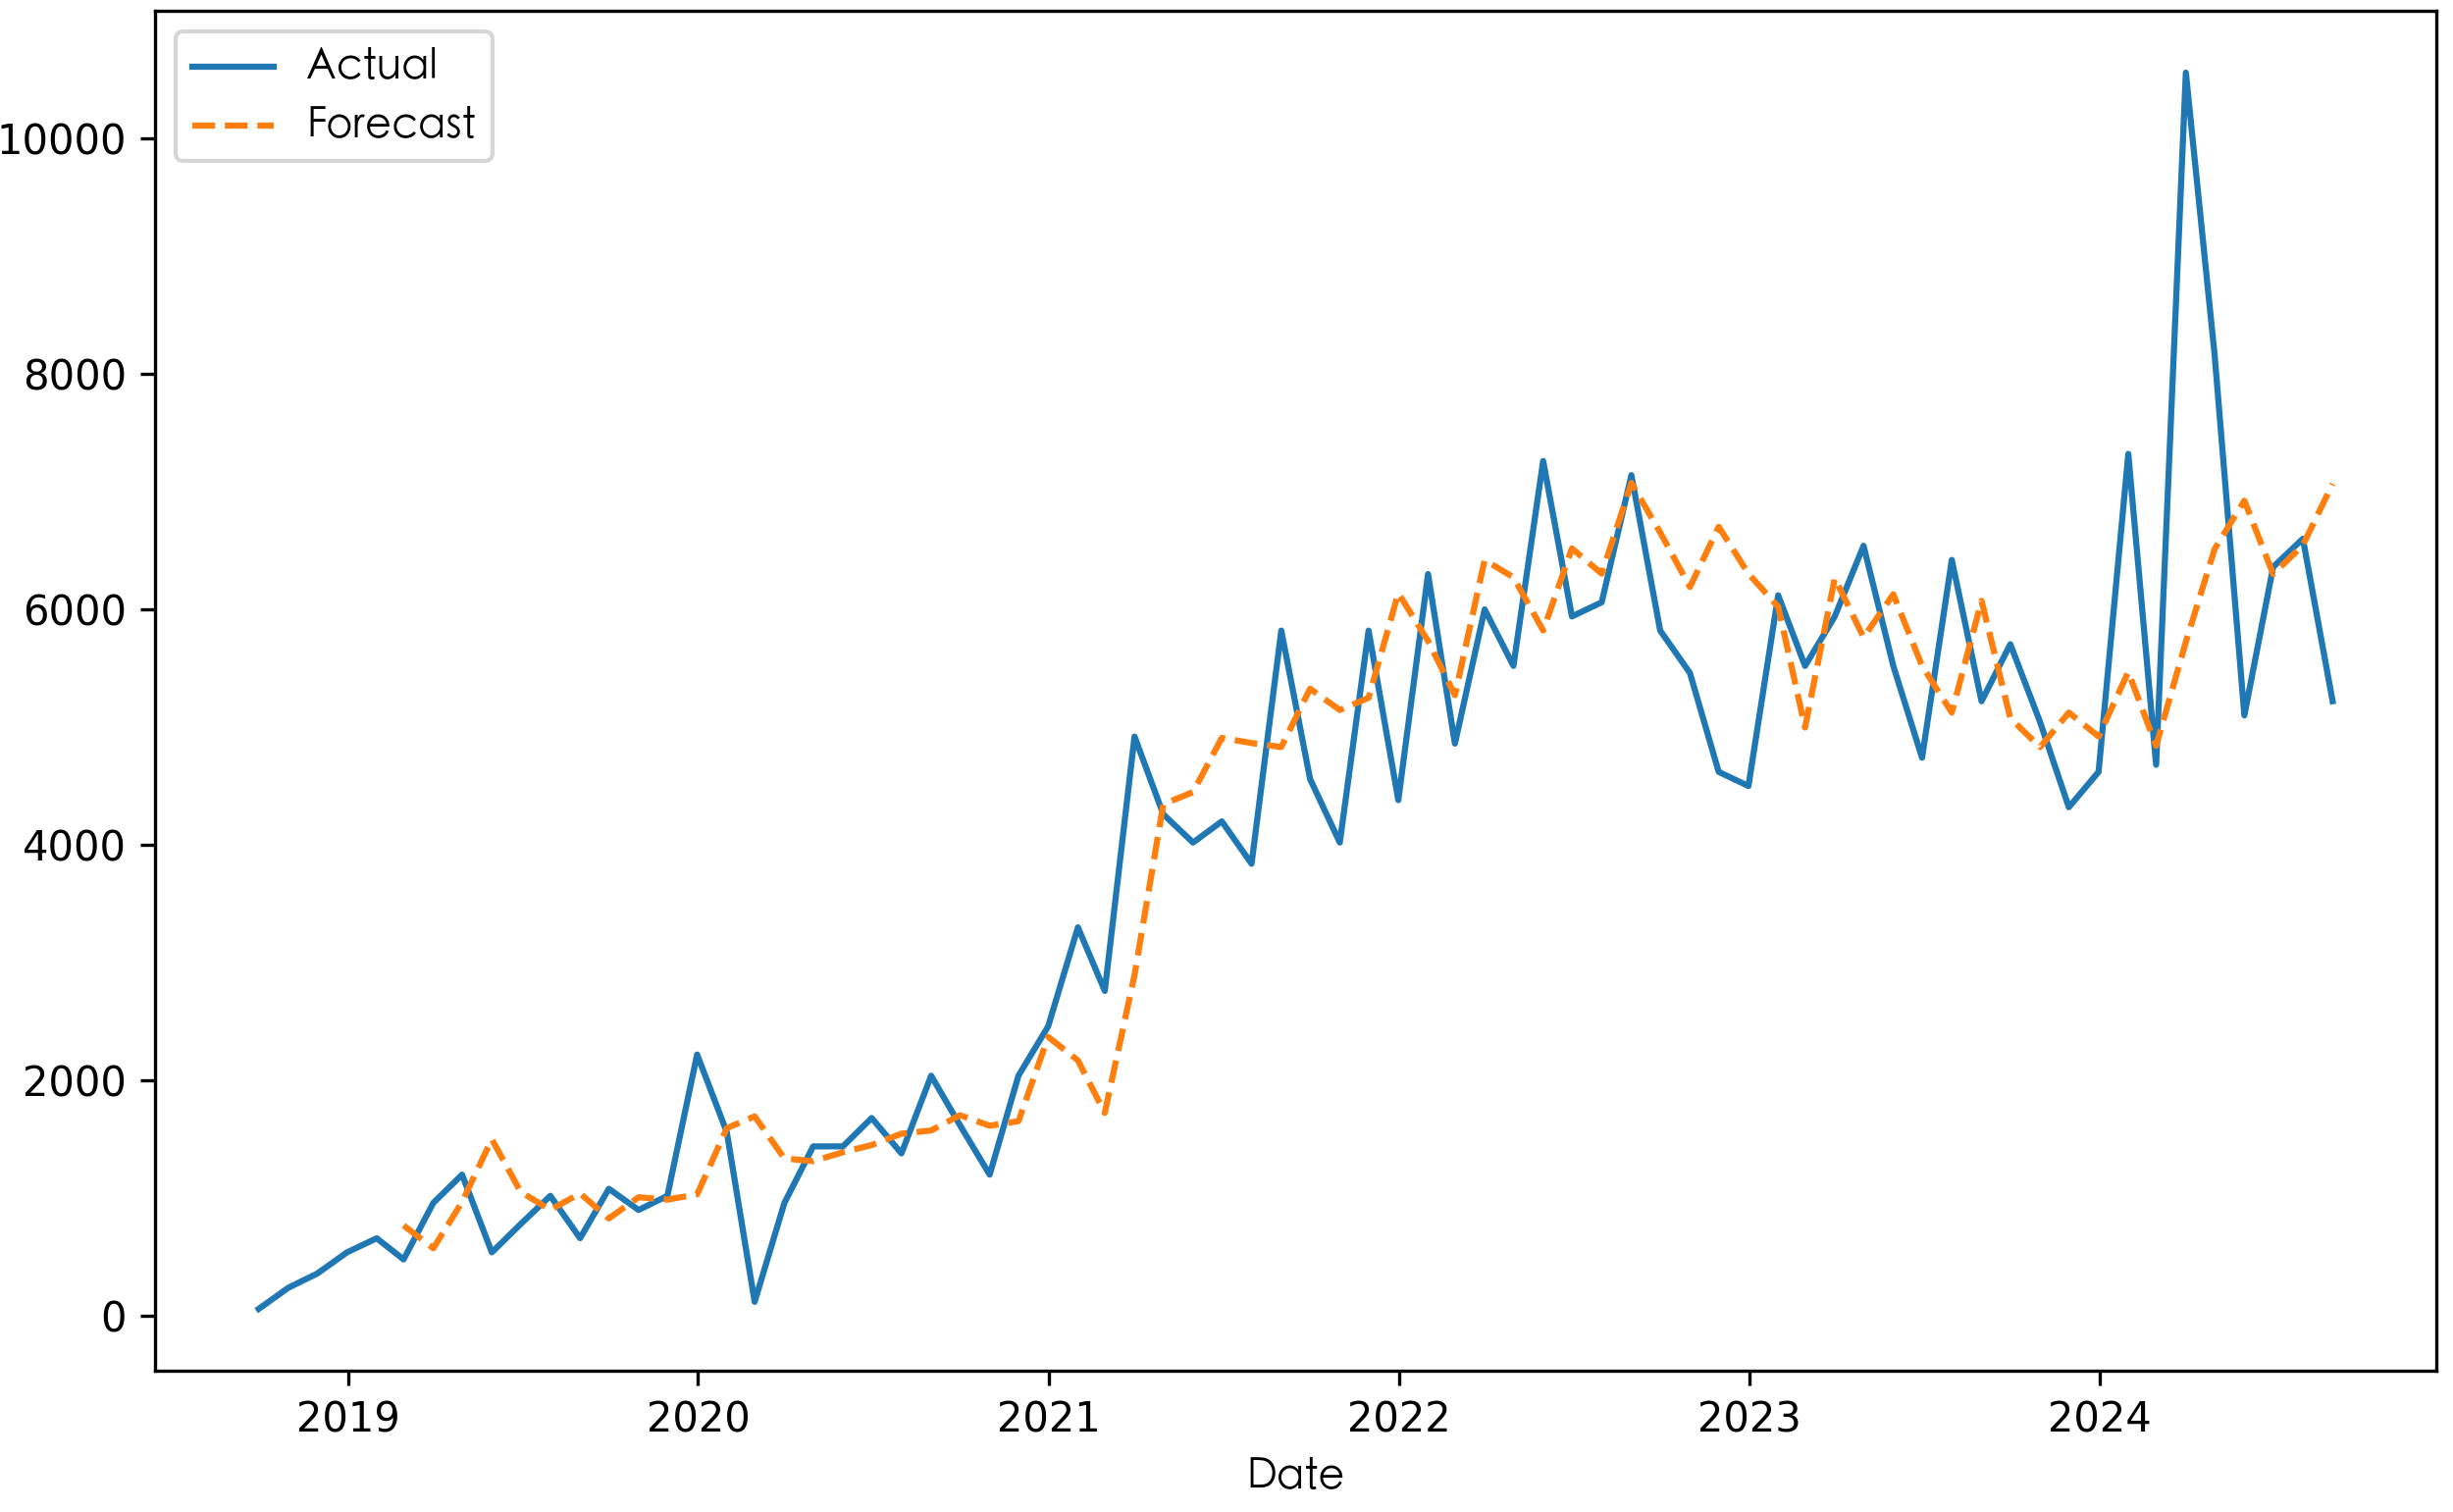
\includegraphics[width=\linewidth]{../Result_Paper/Prophet_Prediction_复方黄柏液涂剂_鲁汉方.png}
\caption{DynamicXSP-P (Prophet) Model Prediction for Compound Phellodendron Liquid by Lu Hanfang.}
\label{fig:phellodendron}
\end{figure}
\item \textbf{Drug:} Shenshuaining Tablets
\begin{itemize}
\item \textbf{Manufacturer:} Shanhaiguan Pharmaceutical
\item \textbf{Metrics:} $R^2 = 0.7348$, SMAPE = 21.86
\end{itemize}
As shown in Figure \ref{fig:shenshuaining}, DynamicXSP-P effectively handled multi-level seasonality and trend variations for Shenshuaining Tablets. Despite the presence of irregular demand fluctuations, the model achieved a moderate $R^2$ of 0.7348 and a relatively low SMAPE of 21.86, suggesting that it captured key structural patterns while maintaining a reasonable prediction error.
\begin{figure}[H]
\centering
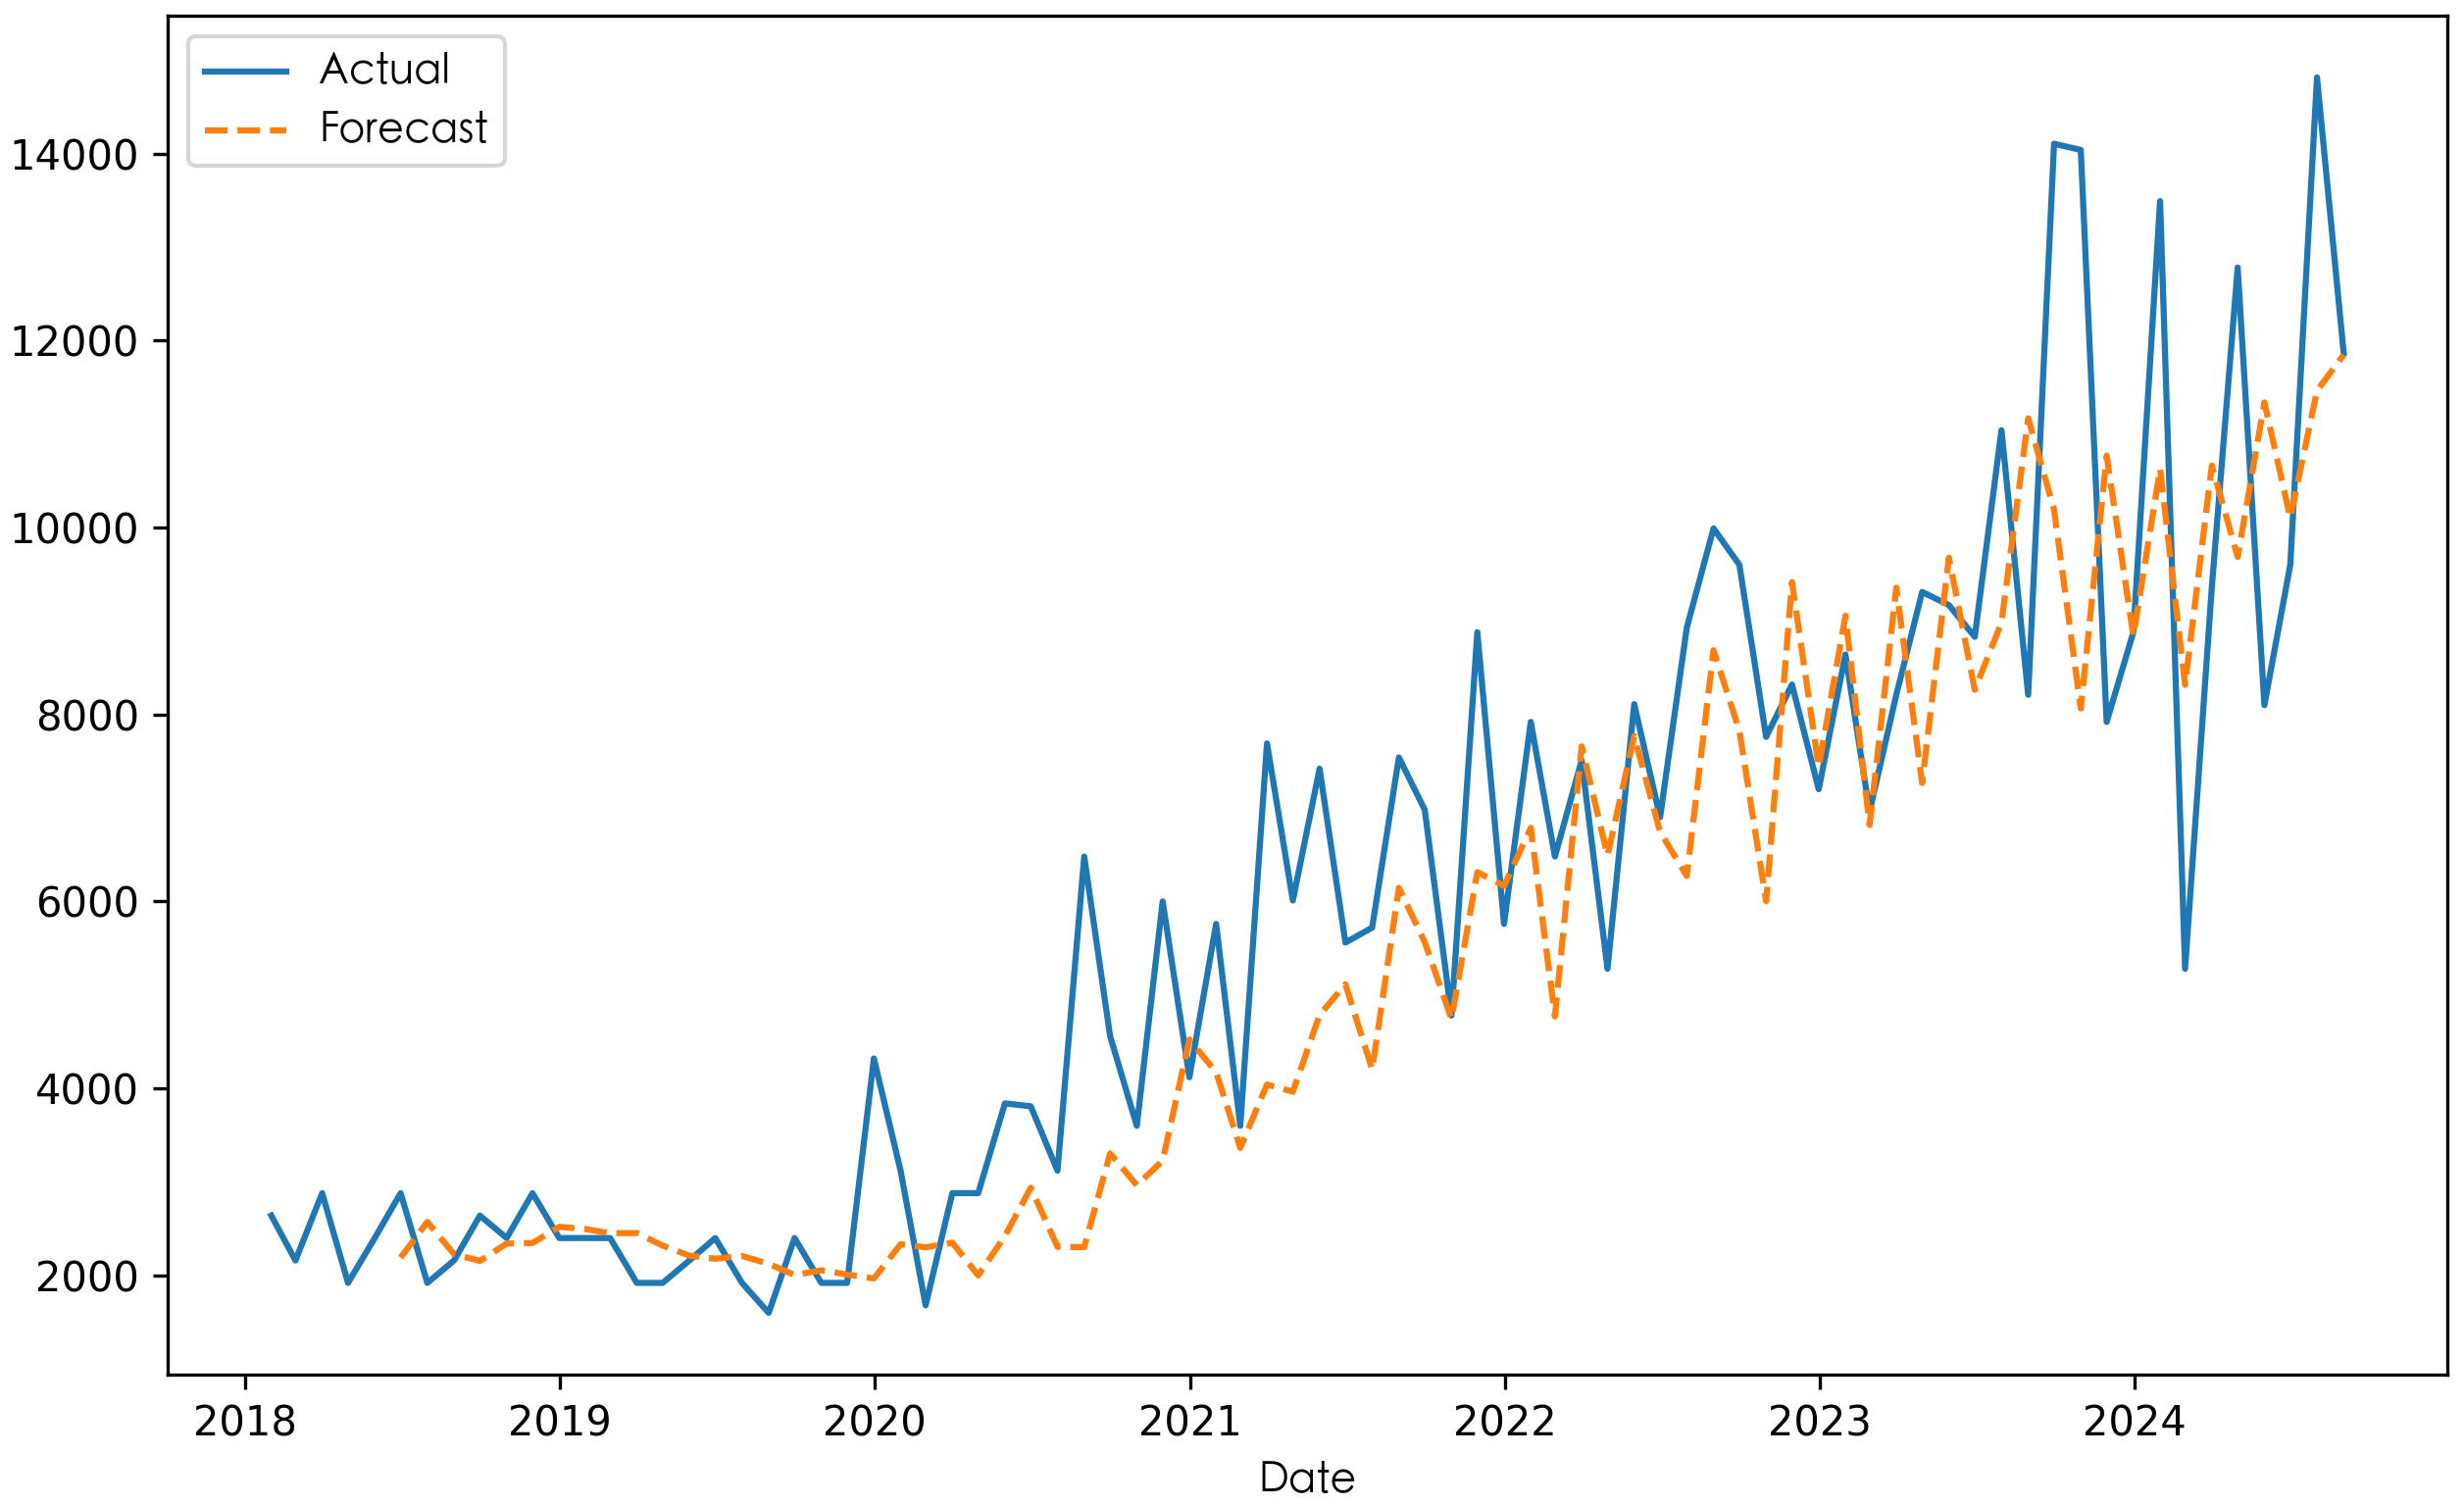
\includegraphics[width=\linewidth]{../Result_Paper/Prophet_Prediction_肾衰宁片_山海关药业.png}
\caption{DynamicXSP-P (Prophet) Model Prediction for Shenshuaining Tablets by Shanhaiguan Pharmaceutical.}
\label{fig:shenshuaining}
\end{figure}
\end{itemize}

\paragraph{DynamicXSP-S (SARIMAX) Model}
\begin{itemize}
\item \textbf{Drug:} Peritoneal Dialysis Solution [Lactate]
\begin{itemize}
\item \textbf{Manufacturer:} Huaren
\item \textbf{Metrics:} $R^2 = 0.8109$, SMAPE = 32.49
\end{itemize}
Figure \ref{fig:peritoneal} shows the DynamicXSP-S (SARIMAX) predictions for Peritoneal Dialysis Solution. The model effectively captured the seasonal patterns and gradual demand decline observed in the historical data. With an $R^2$ of 0.8109, SARIMAX demonstrated strong alignment with actual trends. However, a higher SMAPE of 32.49 suggests that while the model excelled at capturing seasonality, deviations in demand magnitude impacted accuracy.
\begin{figure}[H]
\centering
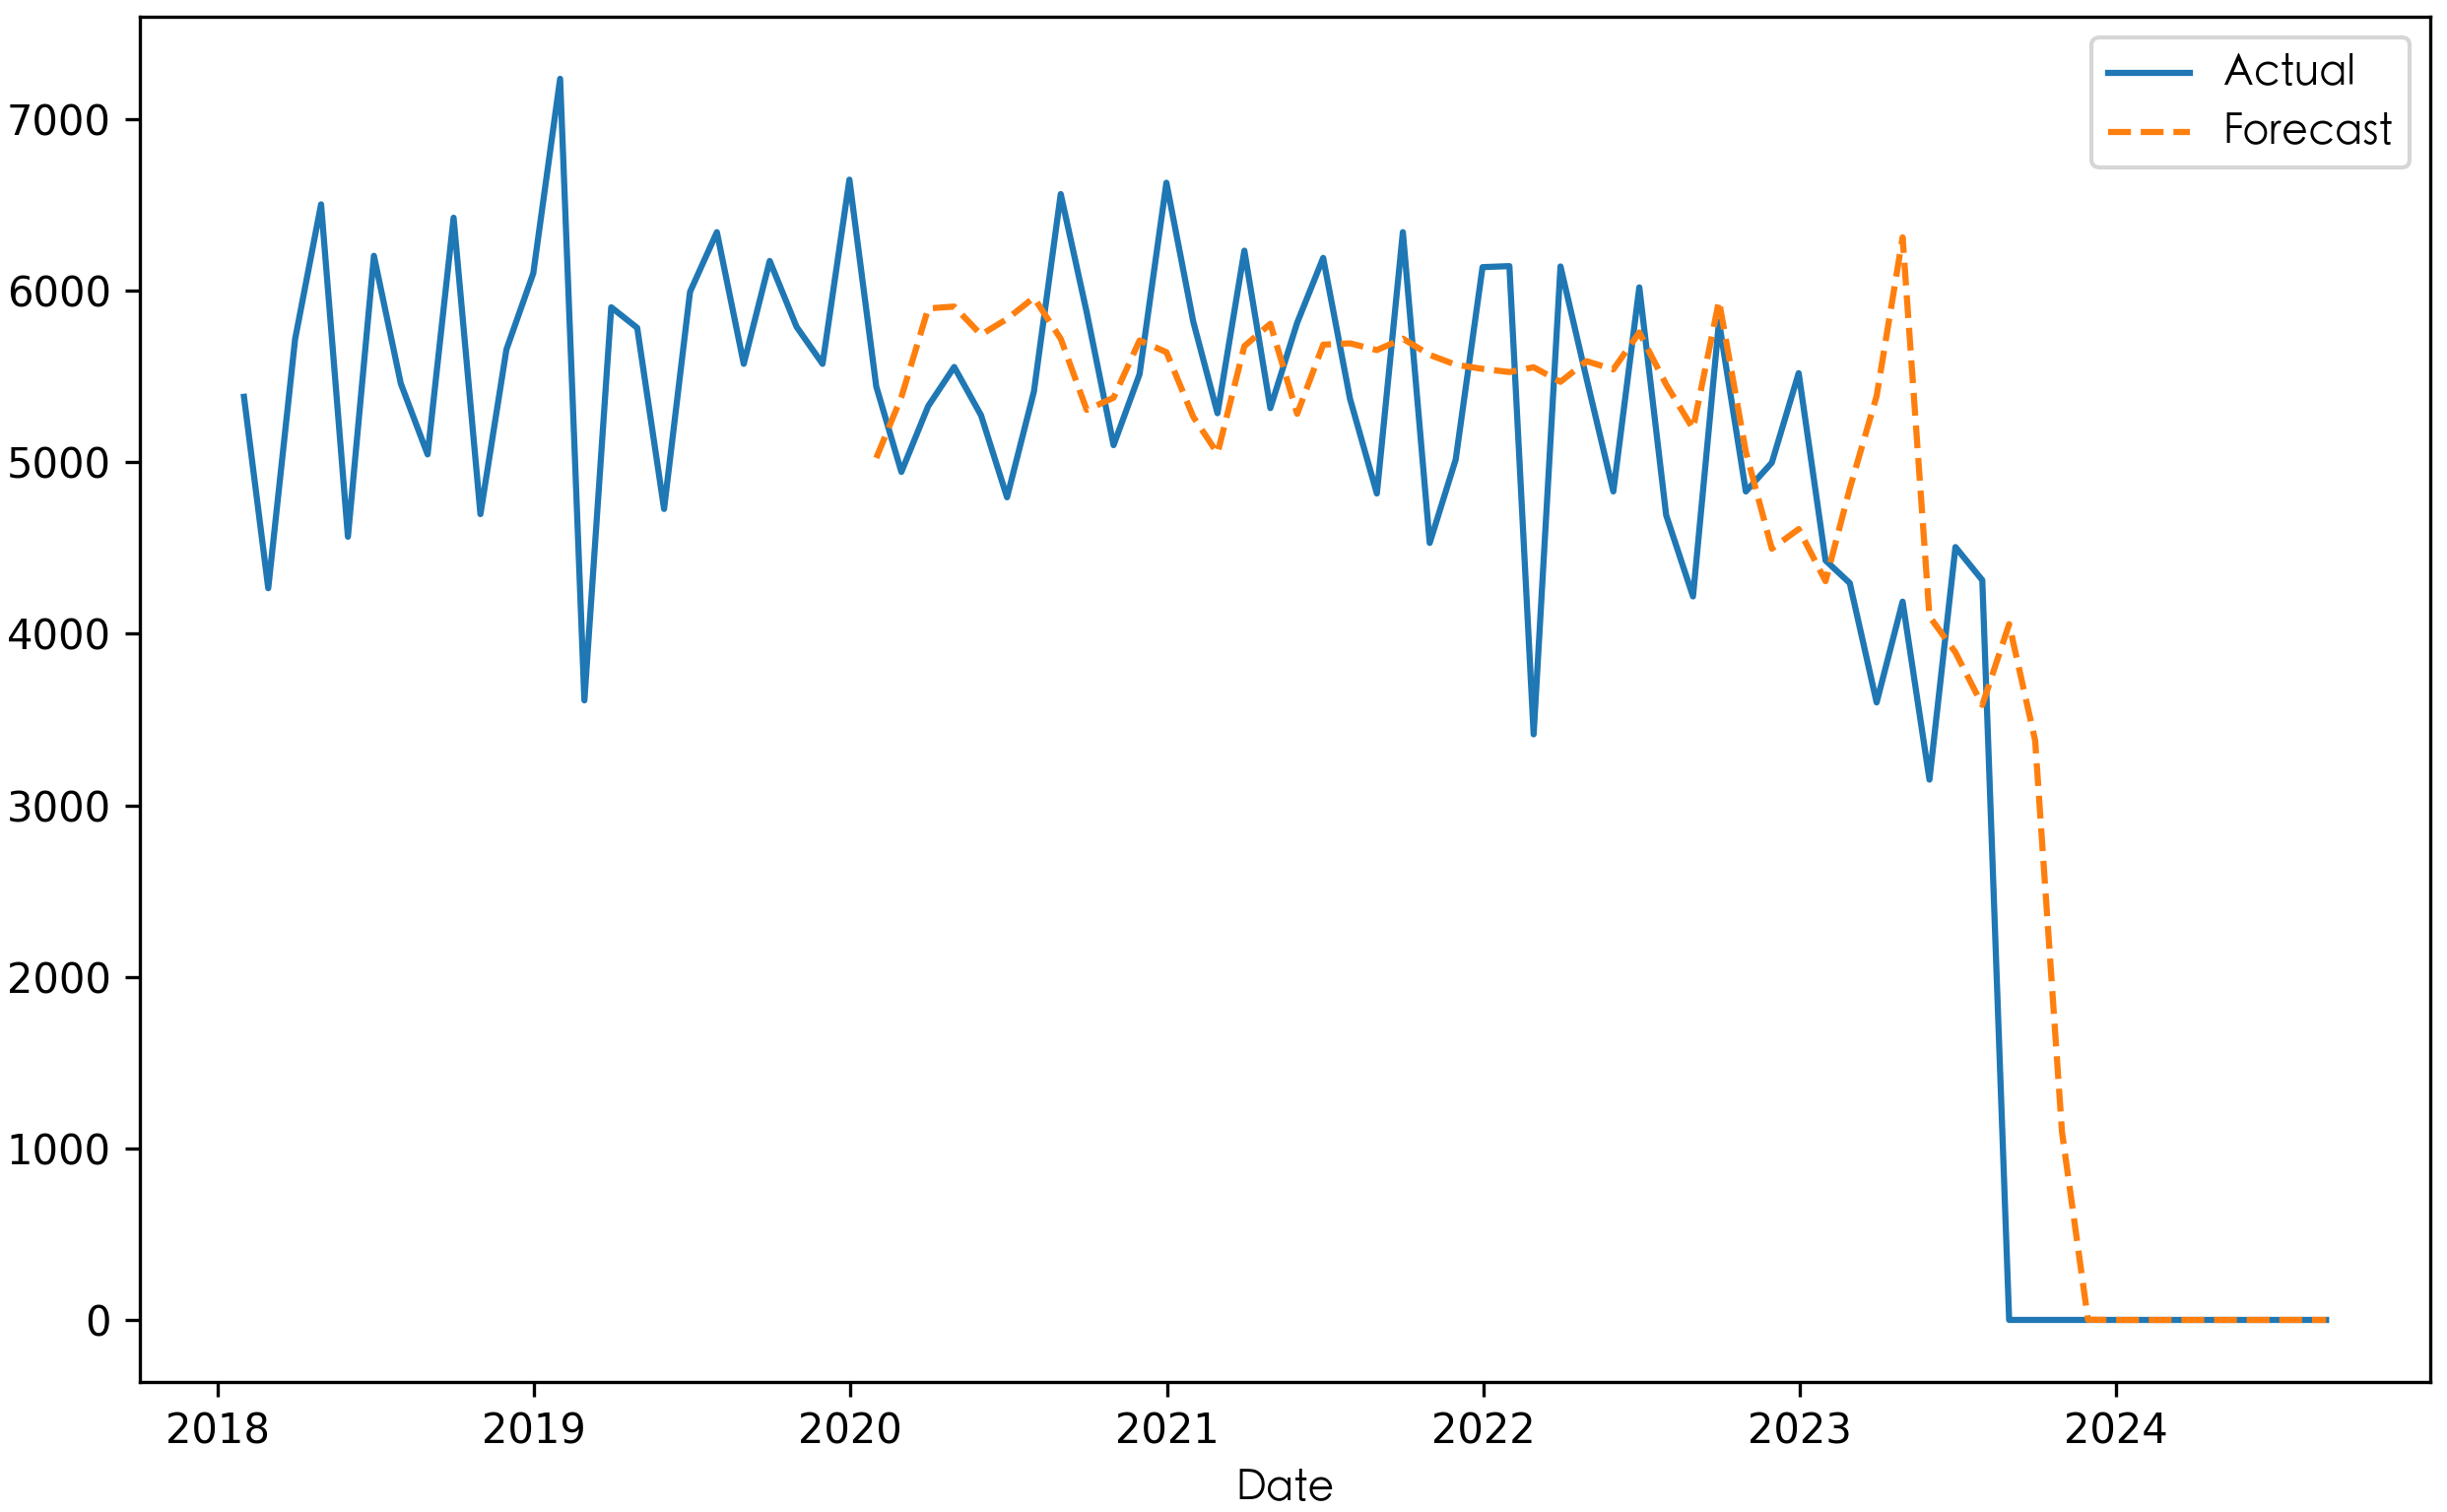
\includegraphics[width=\linewidth]{../Result_Paper/SARIMAX_Prediction_腹膜透析液[乳酸盐]_华仁.png}
\caption{DynamicXSP-S (SARIMAX) Model Prediction for Peritoneal Dialysis Solution by Huaren.}
\label{fig:peritoneal}
\end{figure}
\item \textbf{Drug:} Vitamin B1 Tablets
\begin{itemize}
\item \textbf{Manufacturer:} Xinyi Huanghe
\item \textbf{Metrics:} $R^2 = 0.7345$, SMAPE = 35.37
\end{itemize}
Figure \ref{fig:vitaminb1} presents the forecast for Vitamin B1 Tablets using DynamicXSP-S (SARIMAX). The model successfully identified external influences affecting sales, with an $R^2$ of 0.7345 indicating moderate predictive power. However, the SMAPE of 35.37 highlights that variability in demand led to higher relative errors, reinforcing SARIMAX’s sensitivity to fluctuations.
\begin{figure}[H]
\centering
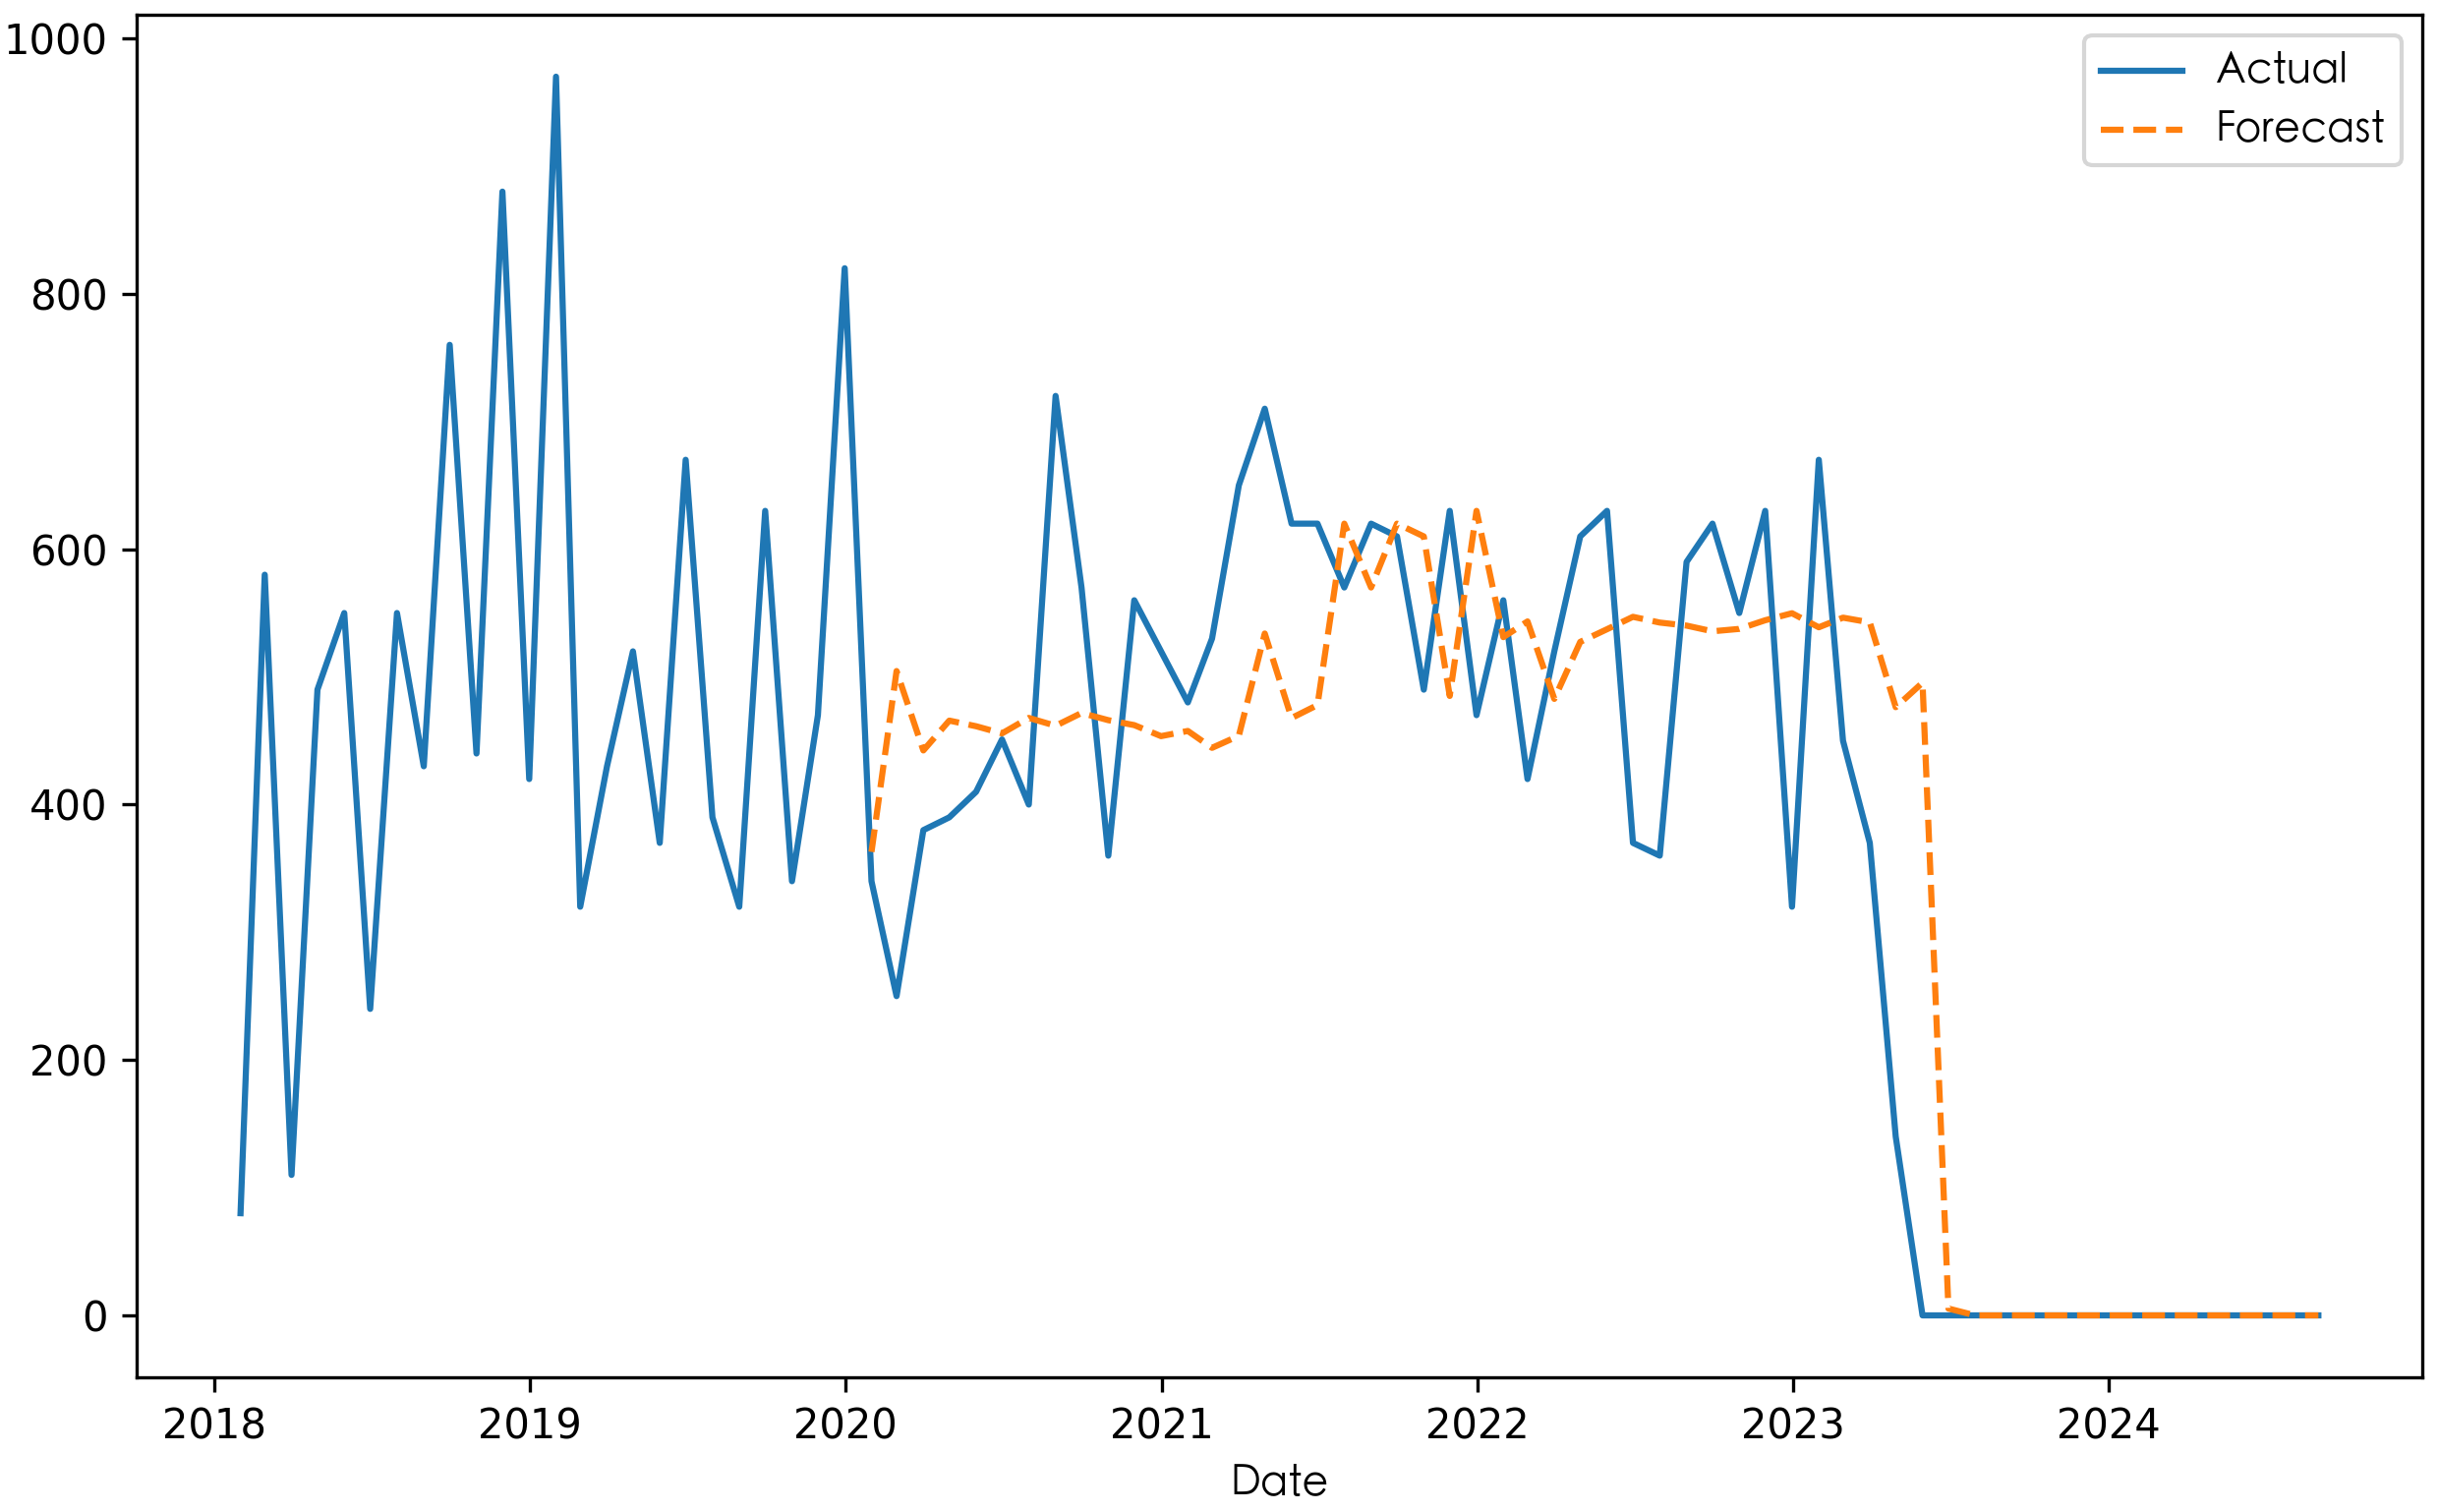
\includegraphics[width=\linewidth]{../Result_Paper/SARIMAX_Prediction_维生素B1片_信谊黄河.png}
\caption{DynamicXSP-S (SARIMAX) Model Prediction for Vitamin B1 Tablets by Xinyi Huanghe.}
\label{fig:vitaminb1}
\end{figure}
\end{itemize}

\subsubsection{Overall Results}

The results highlighted that no single model universally outperformed the others across all cases, underscoring the importance of tailoring each choice of forecasting models to specific data characteristics. DynamicXSP-S (SARIMAX) Model presented superior capability in capturing seasonality influenced by external variables, such as pricing trends and policy changes. DynamicXSP-X (XGBoost) Model excelled in modeling complex, non-linear relationships within the data, making it particularly effective for patterns with high variability. DynamicXSP-P (Prophet) Model performed well in cases with dominant seasonality and long-term trends, such as periodic spikes in drug demand. These findings prove the necessary of DynamicXSP by leveraging the complementary strengths of each single model. 

From a performance metrics perspective, DynamicXSP-X generally achieved the highest $R^2$ scores in datasets with high variability, demonstrating its ability to capture complex dependencies. Meanwhile, DynamicXSP-S provided stable accuracy in structured seasonal data, and DynamicXSP-P maintained competitive SMAPE values in trend-driven cases but showed higher errors in volatile demand patterns. The hybrid approach significantly improved forecasting robustness by dynamically selecting the most suitable model.


The DynamicXSP model analysis reveals several key findings:

\textbf{Long-term Trend Capture}:
\begin{itemize}
\item All models effectively captured the underlying growth trends, with Prophet showing particular strength in long-term pattern recognition.
\item DynamicXSP-S (SARIMAX) Model demonstrated superior performance in capturing gradual trend changes, as evidenced in the insulin device forecasts.
\end{itemize}

\textbf{Seasonal Pattern Recognition}:
\begin{itemize}
\item DynamicXSP-X (XGBoost) Model effectively captured complex seasonal patterns in chronic medication usage.
\item DynamicXSP-S (SARIMAX) Model showed strong performance in regular seasonal variations, particularly in established products.
\end{itemize}

\textbf{Growth Pattern Adaptation}:
\begin{itemize}
\item DynamicXSP-P (Prophet) Model demonstrated superior capability in adapting to emerging growth patterns.
\item DynamicXSP-X (XGBoost) Model showed strong performance in capturing non-linear growth relationships.
\end{itemize}

\subsection{Comparison with Basic Models}

To demonstrate the effectiveness of the DynamicXSP model, we compare it against three baseline models: Prophet, SARIMAX, and XGBoost, each applied without optimizations such as hyperparameter tuning, rolling predictions, or grid search.

The results indicate the baseline models are hard to provide accurate predictions. Compared with DynamicXSP, SMAPE values are notably higher in the baseline models across all cases. Additionally, the baseline models show limited explanatory power, which means an adaptive approach is necessary. Therefore, the DynamicXSP model, which incorporates rolling forecasting, parameter tuning, and additional feature engineering, exhibits significantly improved performance. 

\section{Discussion and Conclusion}

\subsection{Discussion}

The DynamicXSP framework demonstrated reliable and differentiated performance across drug-manufacturer combinations. For example, XGBoost achieved the highest R² in forecasting Mycophenolate Sodium Enteric Tablets (Novartis), accurately capturing irregular and nonlinear fluctuations. In contrast, SARIMAX showed strong seasonal alignment in drugs like Peritoneal Dialysis Solution (Huaren), while Prophet was effective in tracking long-term growth patterns in Compound Phellodendron Liquid (Lu Hanfang). These results benefited from a shared foundation of dynamic temporal features—including lagged consumption values, rolling statistics (mean, std), seasonal encodings (sine/cosine), exponentially weighted moving averages (EWMA), and trend indicators (e.g., percentage change, trend strength)—that adapt to local patterns in each time series. These observations are consistent with recent findings that hybrid modeling frameworks improve accuracy by matching model complexity to specific data regimes rather than relying on a single forecasting architecture. ~\cite{bandara2020}~\cite{petropoulos2020}

The predictions also revealed interpretable trends that aligned with known clinical and policy events. For instance, the demand spike in Mycophenolate Sodium during Q3 2023 coincided with hospital stockpiling activity following regional COVID-19 recovery measures. Similarly, the seasonal drop in Peritoneal Dialysis Solution aligned with national reimbursement policy adjustments in early 2022. These examples reinforce the value of incorporating exogenous signals and rolling recalibration, especially under uncertain procurement behavior~\cite{kwon2023}. Moreover, by surfacing drug-specific temporal dynamics, DynamicXSP provides a granular view of how policy, disease cycles, and manufacturer variation jointly shape pharmaceutical demand—insights not easily captured through fixed-model approaches.

\subsection{Limitations and Future Work}

Despite its advantages, the DynamicXSP framework introduces additional system complexity due to model selection, rolling updates, and feature engineering. However, our experiments suggest that with modular implementation and proper resource management (e.g., limiting grid search space), the framework remains computationally feasible on standard hardware.

In addition, regional variability in drug usage and procurement behaviors poses challenges for model generalization. In countries like China, prescription patterns and hospital purchasing frequencies may vary significantly due to local policy, physician preference, or alternative drug availability. These factors can introduce demand fluctuations that are difficult to fully capture with current exogenous features.

To address these limitations, future work may include:
\begin{itemize}
    \item Incorporating hospital-level metadata (e.g., size, location, tier) and clinical pathway information to enhance feature richness.
    \item Integrating more real-time signals such as public health alerts or sudden price changes to capture demand shocks.
    \item Exploring lightweight Transformer-based architectures as potential substitutes for Prophet or SARIMAX in long-horizon forecasting tasks.
\end{itemize}

\subsection{Conclusion}

This study presents DynamicXSP, a hybrid forecasting framework that integrates SARIMAX, Prophet, and XGBoost with rolling-window forecasting and dynamic feature engineering. The framework adapts model selection to the structure of each time series and demonstrates strong empirical performance across diverse drug-manufacturer combinations. By leveraging the complementary strengths of the three models—SARIMAX for seasonality and exogenous effects, Prophet for trend decomposition, and XGBoost for nonlinear patterns—DynamicXSP enables accurate forecasting under a wide range of demand behaviors.

Beyond predictive accuracy, DynamicXSP provides real-world utility for hospital pharmacy operations. It enhances short- and mid-term demand forecasts, supporting more effective procurement planning, mitigating the risks of shortages or overstocking, and improving supply chain efficiency. Its ability to generalize across datasets with varying seasonality, sparsity, and external drivers makes it particularly well-suited for large-scale deployment in healthcare systems and offers a solid foundation for broader applications in public health analytics and resource optimization.

\section*{Funding}
This research was partially supported by USTC Research Funds of the Double First-Class Initiative (grant no. YD9110002094).

% ========== CONTRIBUTIONS ==========
\section*{Authors' Contributions}

Haizhu Tan: Writing – review and editing, Methodology, Supervision, Resources. Yuxin Fan: Writing – review and editing, Supervision, Methodology, Formal analysis, Conceptualization. Anping Guo: Data collection, Data organization and validation, Resources, Writing – review and editing. Siye Wu: Data analysis and visualization, Writing – initial manuscript draft, Writing – review and editing, Data curation. Chiyu Wei: Data analysis, Writing – manuscript preparation. Zhenzhen Pan: Data collection, Manuscript editing, Funding acquisition.

% ========== CONFLICT OF INTEREST ==========
\section*{Conflicts of Interest}
The authors declare no competing interests. The authors declare that they have no known competing financial interests or personal relationships that could have appeared to influence the work reported in this paper.

% ========== CODE AVAILABILITY ==========
\section*{Code Availability}
All code used in this study is available at: \url{https://github.com/yx-fan/medicine_sale_prediction}

% ========== REFERENCES ==========

\begin{thebibliography}{99}

\bibitem{who2016}
World Health Organization. WHO Drug Information. 2016;30(2):180-189.

\bibitem{fda2021}
U.S. Food and Drug Administration. Drug Shortages. 2021. Available: \url{https://www.fda.gov/drugs/drug-safety-and-availability/drug-shortages}

\bibitem{bhat2024optimizing}
Bhat SS, Satheesh SS, Srihari VR, Bidrohi AB, Prabhune A. Optimizing medication access in public healthcare centers: A machine learning stochastic model for inventory management and demand forecasting in primary health services. Proceedings of the 2024 International Conference on Intelligent and Innovative Technologies in Computing, Electrical and Electronics (IITCEE); 2024.

\bibitem{koala2021factors}
Koala D, Yahouni Z, Alpan G, Frein Y. Factors influencing drug consumption and prediction methods. CIGI-Qualita: Conférence Internationale Génie Industriel QUALITA. Grenoble, France; 2021.

\bibitem{taylor2018forecasting}
Taylor SJ, Letham B. Forecasting at scale. The American Statistician. 2018;72(1):37-45. doi:10.1080/00031305.2017.1380080

\bibitem{chen2016xgboost}
Chen T, Guestrin C. XGBoost: A scalable tree boosting system. Proceedings of the 22nd ACM SIGKDD International Conference on Knowledge Discovery and Data Mining. 2016:785-794.

\bibitem{meng2021comparative}
Meng J, Zhang Q, Li X. Comparative analysis of Prophet and LSTM models in drug sales forecasting. Journal of Physics: Conference Series. 2021;1910(1):012059.

\bibitem{xu2019hybrid}
Xu W, Wang Y, Zhao J. A hybrid modelling method for time series forecasting based on a linear regression model and deep learning. Applied Intelligence. 2019;49(7):2875-2888.

\bibitem{siddiqui2021hybrid}
Siddiqui R, Khan A, Ahmed M. A Hybrid Demand Forecasting Model for Greater Forecasting Accuracy: The Case of the Pharmaceutical Industry. Supply Chain Forum: An International Journal. 2021;22(3):1-13.

\bibitem{rathipriya2022pharma}
Rathipriya R, Saranya M, Ramkumar K. Demand Forecasting Model for Time-Series Pharmaceutical Data Using Neural Networks. Neural Computing and Applications. 2022;35:1945-1957.

\bibitem{lee2019}
Lee C, Kim J, Park D. Predicting drug utilization using machine learning: An empirical study. Health Informatics Journal. 2019;25(3):1065-1076.

\bibitem{hyndman2006accuracy}
Hyndman RJ, Koehler AB. Another look at measures of forecast accuracy. International Journal of Forecasting. 2006;22(4):679-688. doi:10.1016/j.ijforecast.2006.03.001

\bibitem{papadopoulos2024}
Papadopoulos A. The impact of climatic factors on respiratory pharmaceutical demand: A comparison of forecasting models for Greece. arXiv preprint arXiv:2505.10642. 2024.

\bibitem{li2023}
Li Z, Wang Y, Liu H. A comparative study of SARIMA, Prophet, XGBoost and LSTM models for medical demand forecasting. Journal of Healthcare Engineering. 2023;2023:1-11.

\bibitem{zhang2021}
Zhang Y, Chen L, Wang M. Hybrid models for time series forecasting in healthcare: A systematic review. Artificial Intelligence in Medicine. 2021;115:102072.

\bibitem{box2015}
Box GEP, Jenkins GM, Reinsel GC, Ljung GM. Time Series Analysis: Forecasting and Control. 5th ed. Hoboken, NJ: Wiley; 2015.

\bibitem{kwarteng2024prophet}
Kwarteng SB, Andreevich PA. Comparative Analysis of ARIMA, SARIMA and Prophet Model in Forecasting. Research \& Development. 2024;5(4):110-120. doi:10.11648/j.rd.20240504.13

\bibitem{liu2020}
Liu B, Zhao Y, Sun K. Rolling window analysis in healthcare forecasting. International Journal of Forecasting. 2020;36(2):654-666.

\bibitem{hyndman2018}
Hyndman RJ, Athanasopoulos G. Forecasting: Principles and Practice. 2nd ed. Melbourne, Australia: OTexts; 2018.

\bibitem{chen2020}
Chen X, Hu J. Multivariate time series forecasting using dynamic models in hospital logistics. Computers in Biology and Medicine. 2020;118:103636.

\bibitem{bandara2020}
Bandara T, Bergmeir C, Smyl S. Forecasting across time series databases using recurrent neural networks on groups of similar series: A clustering approach. Expert Systems with Applications. 2020;140:112896.

\bibitem{petropoulos2020}
Petropoulos F, Makridakis S, Spiliotis E. Statistical and machine learning forecasting methods: Concerns and ways forward. PLOS ONE. 2020;15(3):e0229287.

\bibitem{kwon2023}
Kwon R, Murdock CP, Goh M. Pharmaceutical supply chain disruptions during public health emergencies: A review and proposed framework. Health Systems. 2023;12(1):1-15.

\end{thebibliography}


\raggedbottom  % 允许页面填充不均匀,减少空白

\appendix
\section{Sample Selection Algorithm}
\label{appendix:sample-selection}

The following pseudocode outlines the sample selection process used to ensure the quality and relevance of the dataset for modeling tasks:

\begin{algorithm}[H]
\caption{Sample Selection Algorithm}
\begin{algorithmic}[1]
\Require Cleaned data $df$, configuration thresholds $\text{config}$
\Ensure Filtered dataset $final\_df$
\State $final\_df \gets \emptyset$
\For{each unique combination of drug name and manufacturer $(d, m)$ in $df$}
    \State $group\_data \gets$ subset of $df$ for $(d, m)$
    \If{length of $group\_data < \text{config.min\_months}$ \textbf{or} sum of consumption $= 0$}
        \State \textbf{Skip group} \Comment{Insufficient or sparse data}
    \EndIf
    \State $non\_zero\_ratio \gets$ proportion of non-zero consumption in $group\_data$
    \If{$non\_zero\_ratio < \text{config.sparsity\_threshold}$}
        \State \textbf{Skip group} \Comment{Data too sparse}
    \EndIf
    \State $acf\_values \gets$ autocorrelation function of consumption in $group\_data$
    \If{$\max(acf\_values[1:]) < \text{config.min\_acf\_threshold}$}
        \State \textbf{Skip group} \Comment{Insufficient autocorrelation}
    \EndIf
    \If{no start date $\geq \text{config.min\_start\_date}$ in $group\_data$}
        \State \textbf{Skip group} \Comment{No recent data}
    \EndIf
    \State $variance \gets$ variance of consumption in $group\_data$
    \If{$variance < \text{config.min\_variance\_threshold}$}
        \State \textbf{Skip group} \Comment{Variance too low}
    \EndIf
    \State $missing\_ratio \gets$ maximum missing ratio for features in $group\_data$
    \If{$missing\_ratio > \text{config.max\_missing\_ratio}$}
        \State \textbf{Skip group} \Comment{Feature missing data too high}
    \EndIf
    \State $skewness \gets$ skewness of consumption in $group\_data$
    \If{$|skewness| > \text{config.max\_skewness}$}
        \State \textbf{Skip group} \Comment{Target variable too skewed}
    \EndIf
    \State $correlation \gets$ correlation of consumption with lagged features in $group\_data$
    \If{$|correlation| < \text{config.min\_correlation}$}
        \State \textbf{Skip group} \Comment{Insufficient correlation with features}
    \EndIf
    \State $final\_df \gets final\_df \cup group\_data$
\EndFor
\State \Return $final\_df$
\end{algorithmic}
\end{algorithm}

\end{document}
